\documentclass[preprint,12pt,review]{elsarticle}
\usepackage{amsmath}
\usepackage{amssymb}
\usepackage{booktabs}
\usepackage{siunitx}
\usepackage{graphicx}
\usepackage{hyperref}
\usepackage{textcomp}
\usepackage{xcolor}
\usepackage{multirow}
\usepackage{array}
\usepackage{lineno}
\usepackage{tikz}
\usepackage{pgfplots}
\usetikzlibrary{arrows.meta,positioning,shapes.geometric,fit,backgrounds,calc,patterns,decorations.markings}
\pgfplotsset{compat=1.18}

%% Maturity symbols for taxonomy table
\newcommand{\fullcirc}[1]{\textcolor{green!60!black}{\textbullet\textbullet\textbullet}}
\newcommand{\halfcirc}[1]{\textcolor{orange!80!black}{\textbullet\textbullet}}
\newcommand{\emptycirc}[1]{\textcolor{red!60!black}{\textbullet}}
\modulolinenumbers[5]
\sisetup{detect-all, group-separator={,}, output-decimal-marker={.}, separate-uncertainty=true}
\journal{Renewable and Sustainable Energy Reviews}

\begin{document}
\begin{frontmatter}
\title{Foundation Models for Clean Energy Systems: A Systematic Review and Deployment Framework}

\author[ox]{Jianou Jiang\corref{cor1}}
\ead{jianou.jiang@eng.ox.ac.uk}
\author[ox2]{Budimir Rosic}
\ead{budimir.rosic@eng.ox.ac.uk}

\cortext[cor1]{Corresponding author.}

\affiliation[ox]{organization={Department of Engineering Science, University of Oxford},
  addressline={Parks Road}, city={Oxford}, postcode={OX1 3PJ}, country={United Kingdom}}
\affiliation[ox2]{organization={Department of Engineering Science, University of Oxford},
  addressline={Osney Mead, Botley}, city={Oxford}, postcode={OX2 0ES}, country={United Kingdom}}

\begin{abstract}
Foundation models---large-scale neural networks pre-trained on broad data and adaptable to diverse downstream tasks---have transformed natural language processing, computer vision, and scientific computing. Their application to clean energy systems, however, remains fragmented and lacks a unifying framework. This paper presents a comprehensive scoping review, guided by the PRISMA-ScR framework, that maps foundation model capabilities onto clean energy operations spanning hydropower, wind energy, solar photovoltaics, and ecological monitoring at energy infrastructure sites. Through structured searches of Web of Science, Scopus, IEEE Xplore, arXiv, and Google Scholar, we identify and synthesise 31 application studies on foundation models in clean energy, published between January 2019 and February 2026. A large-scale bibliometric analysis of 3{,}645 classified papers from OpenAlex reveals exponential publication growth (doubling time 1.3 years, $R^2 = 0.95$), geographic concentration in China and the USA, and critical reproducibility gaps (only 5.5\% of papers share code). We propose a structured taxonomy that cross-references five foundation model paradigms (large language models, vision-language models, time-series foundation models, diffusion models, and multimodal transformers) against seven clean energy task categories. Building on this taxonomy, we introduce the Clean Energy Foundation Model Deployment Framework (CEFMDF), a four-layer architecture---Perception, Reasoning, Decision, and Interface---that specifies how foundation models integrate with existing SCADA and EMS infrastructure. Five benchmark experiments---time-series forecasting with Chronos, zero-shot solar panel inspection with CLIP, LLM energy Q\&A, RAG pipeline evaluation, and a reproducibility audit---provide original quantitative evidence on FM capabilities and limitations for energy applications. This review provides energy engineers and policymakers with a data-driven roadmap for deploying foundation models in clean energy infrastructure.
\end{abstract}

\begin{keyword}
foundation models \sep large language models \sep clean energy \sep hydropower \sep wind energy \sep solar energy \sep systematic review \sep deployment framework \sep ecological monitoring
\end{keyword}

\end{frontmatter}
\linenumbers

%%====================================================================
%% SECTION 1: INTRODUCTION
%%====================================================================
\section{Introduction}
\label{sec:introduction}

The global clean energy transition demands increasingly sophisticated tools for managing complex, heterogeneous data streams across power generation, transmission, and ecological stewardship. Hydropower reservoirs produce multi-decadal hydrological records alongside real-time turbine vibration signals; wind farms generate terabytes of SCADA data combined with meteorological reanalysis fields and drone inspection imagery; solar installations integrate satellite-derived irradiance maps with panel-level thermal signatures; and ecological monitoring at energy infrastructure sites spans acoustic recordings, underwater camera feeds, and satellite vegetation indices. No single conventional machine learning model---trained from scratch on a narrow, site-specific dataset---handles this diversity adequately \cite{wang2023dl_renewable_forecasting}.

Foundation models (FMs) offer a fundamentally different paradigm. Defined by Bommasani et al. \cite{bommasani2021opportunities} as models ``trained on broad data at scale and adaptable to a wide range of downstream tasks,'' FMs exhibit emergent capabilities absent from their smaller predecessors: in-context learning, zero-shot generalisation, chain-of-thought reasoning, and cross-modal grounding \cite{wei2022emergent}. These capabilities map directly onto unsolved problems in clean energy operations---multi-source data fusion, rapid adaptation to new plant sites without costly retraining, natural language explainability for operator decision support, and ecological monitoring at scale with limited labelled data.

Yet despite rapid advances in foundation model architectures---from GPT-4 \cite{achiam2023gpt4} and LLaMA \cite{touvron2023llama2} in language to CLIP \cite{radford2021learning} and Segment Anything \cite{kirillov2023sam} in vision, and from TimeGPT to Moirai \cite{woo2024moirai} in time series---their adoption in clean energy remains fragmented. Existing review articles address either traditional deep learning for energy forecasting \cite{wang2023dl_renewable_forecasting, ahmed2020wind_forecasting_review} or large language models for general industrial applications \cite{zhao2023llm_survey, minaee2024llm_survey}, but none systematically maps the full spectrum of foundation model capabilities onto the specific technical challenges of clean energy operations and ecological monitoring.

This paper addresses that gap with five contributions:

\begin{enumerate}
\item A \textbf{comprehensive scoping review} (2019--2026), guided by the PRISMA-ScR framework \cite{tricco2018prisma_scr, page2021prisma}, synthesising 31 application studies with transparent methodology and eligibility criteria.

\item A \textbf{large-scale bibliometric analysis} of 3{,}645 classified FM+energy papers from OpenAlex, quantifying publication growth, geographic distribution, thematic structure, and reproducibility gaps.

\item A \textbf{structured taxonomy} cross-referencing five foundation model paradigms against seven clean energy task categories, with data-driven maturity assessment from the bibliometric corpus.

\item The \textbf{Clean Energy Foundation Model Deployment Framework (CEFMDF)}, a four-layer architecture (Perception--Reasoning--Decision--Interface) specifying how foundation models integrate with existing SCADA/EMS infrastructure.

\item \textbf{Five benchmark experiments}---time-series forecasting, LLM energy Q\&A, VLM zero-shot inspection, RAG pipeline evaluation, and a reproducibility audit---providing original quantitative evidence on FM capabilities for energy applications.
\end{enumerate}

The remainder of this paper is organised as follows. Section~\ref{sec:methodology} describes the scoping review protocol. Section~\ref{sec:bibliometrics} presents the bibliometric analysis. Section~\ref{sec:background} provides a technical primer on foundation model architectures. Section~\ref{sec:taxonomy} presents the taxonomy. Section~\ref{sec:framework} introduces the CEFMDF. Sections~\ref{sec:hydro}--\ref{sec:ecological} analyse domain-specific applications. Section~\ref{sec:benchmarks} reports the benchmark experiments. Section~\ref{sec:challenges} discusses challenges and a research agenda, and Section~\ref{sec:conclusions} concludes.

%%====================================================================
%% SECTION 2: REVIEW METHODOLOGY
%%====================================================================
\section{Review Methodology}
\label{sec:methodology}

This scoping review follows the PRISMA extension for Scoping Reviews (PRISMA-ScR) \cite{tricco2018prisma_scr} and the scoping study framework of Arksey and O'Malley \cite{arksey2005scoping}, supplemented by the systematic literature review guidelines for engineering research \cite{kitchenham2007guidelines}. A scoping review was chosen over a full systematic review because the field of foundation models in clean energy is nascent and rapidly evolving, with heterogeneous study designs, outcome measures, and validation approaches that preclude quantitative meta-analysis. The scoping review methodology is well suited to mapping the extent and nature of research activity, identifying gaps, and informing future research directions \cite{page2021prisma}.

\subsection{Search strategy}
\label{subsec:search_strategy}

Five electronic databases were searched: Web of Science (WoS), Scopus, IEEE Xplore, arXiv, and Google Scholar. Targeted citation chasing (forward and backward) was conducted from key anchor papers in each domain. The search was executed between December 2025 and February 2026 and covered publications from January 2019 to February 2026. The start date of 2019 was chosen to coincide with the publication of BERT \cite{devlin2019bert}, which established the pre-train--fine-tune paradigm that defines foundation models; seminal architecture papers from 2017--2018 (e.g., the Transformer \cite{vaswani2017attention}) were included as foundational references.

The search string combined foundation model terminology with clean energy domain terms:

\begin{quote}
\texttt{("foundation model" OR "large language model" OR "LLM" OR "vision-language model" OR "multimodal model" OR "generative AI" OR "GPT" OR "pretrained transformer" OR "time series foundation model") AND ("clean energy" OR "renewable energy" OR "hydropower" OR "wind energy" OR "wind power" OR "solar energy" OR "photovoltaic" OR "energy forecasting" OR "turbine" OR "ecological monitoring" OR "reservoir" OR "dam operations")}
\end{quote}

The string was adapted for each database's syntax. Boolean operators and field restrictions (title, abstract, keywords) were applied consistently. Given the rapid pace of foundation model research, arXiv preprints with demonstrated community engagement (citations $\geq 5$ or accepted at a peer-reviewed venue by February 2026) were included alongside journal and conference publications. We note that the arXiv citation threshold may create a bias against the most recent work (2025--2026), where accumulating $\geq 5$ citations within months is unlikely; this is partially mitigated by the venue-acceptance criterion.

\textit{Databases not included:} CNKI (China National Knowledge Infrastructure) was not included in the formal search despite this review's emphasis on Chinese AI deployment, due to the English-language scope of the primary search and access constraints. Chinese-language FM application studies published in domestic journals may therefore be underrepresented; this is acknowledged as a limitation. Studies from Chinese research groups published in English-language venues were captured through the five databases listed above.

\textit{Search completeness check:} As a validation of search coverage, we compared the included study set against the reference lists of the two most relevant competing reviews---Zhou et al. \cite{zhou2024llm_energy_review} and Lotfi et al. \cite{lotfi2024generativeai_energy}. All FM-specific application studies cited in those reviews that met our eligibility criteria were also identified by our search. The citation chasing process additionally identified 7 studies not referenced in either competing review, primarily in the ecological monitoring and hydropower domains.

\subsection{Eligibility criteria}
\label{subsec:eligibility}

Studies were included if they met all of the following criteria:
\begin{itemize}
\item Applied, proposed, or evaluated a foundation-model-class architecture (as defined by Bommasani et al. \cite{bommasani2021opportunities}: pre-trained on large-scale data with demonstrated adaptability to downstream tasks via prompting, fine-tuning, or retrieval-augmented generation) in the context of clean energy operations or ecological monitoring at energy infrastructure sites.
\item Published in English or Chinese in a peer-reviewed journal, conference proceedings, or as a substantive arXiv preprint with community engagement.
\item Provided sufficient methodological detail for assessment (excluding editorials, short abstracts, and position papers without technical content).
\end{itemize}

Studies were excluded if they:
\begin{itemize}
\item Used only classical machine learning or standard deep learning (LSTM, CNN, vanilla Transformer trained from scratch on a single dataset) without any foundation model component.
\item Focused exclusively on nuclear energy, oil and gas, energy trading/markets, or transmission-level grid stability.
\item Were duplicate publications (the most complete version was retained).
\end{itemize}

A critical distinction was enforced: a Transformer-based model trained from scratch on a single energy dataset (e.g., a custom Transformer for wind speed forecasting) was classified as standard deep learning, not a foundation model. Foundation model status required evidence of large-scale pre-training on diverse data and demonstrated transfer capability. Models such as PatchTST \cite{nie2023patchtst} qualify as foundation models when pre-trained on large multi-domain corpora (as in MOMENT \cite{goswami2024moment}) but not when trained from scratch on a single energy dataset.

\subsection{Screening and charting}
\label{subsec:screening}

Fig.~\ref{fig:prisma} summarises the screening process following PRISMA-ScR conventions. The initial database searches and citation chasing yielded approximately 427 candidate records. After removing approximately 138 duplicates, 289 unique records were screened at the title/abstract level by the first author, of which approximately 198 were excluded (not foundation-model class, wrong energy domain, or insufficient methodological detail). The remaining 91 records were assessed at full-text level against the eligibility criteria; 60 were excluded (standard deep learning only, out of scope, or duplicate publications), yielding \textbf{31 included application studies} that specifically apply foundation-model-class architectures to clean energy operations or ecological monitoring at energy sites. These 31 studies form the basis of the synthesis presented in Sections~\ref{sec:taxonomy}--\ref{sec:ecological}. The bibliography additionally contains 80 foundational architecture papers, review methodology references, competing surveys, and background references that contextualise but are not themselves included application studies.

\subsection{Data charting and coding}
\label{subsec:coding}

Each included study was charted along six dimensions, following PRISMA-ScR terminology:

\begin{enumerate}
\item \textbf{Energy domain}: hydropower, wind, solar, ecological monitoring, or multi-domain.
\item \textbf{Foundation model type}: large language model (LLM), vision-language model (VLM), time-series foundation model (TSFM), diffusion model, multimodal transformer, or hybrid.
\item \textbf{Deployment strategy}: zero-shot prompting, few-shot prompting, fine-tuning (full or parameter-efficient via LoRA \cite{hu2022lora}), retrieval-augmented generation (RAG) \cite{lewis2020rag}, agent-based framework, or hybrid.
\item \textbf{Task type}: forecasting, fault detection, anomaly narration, operational Q\&A, image-based inspection, data augmentation, planning/scheduling, or other.
\item \textbf{Validation approach}: quantitative benchmark with held-out test set, case study or proof of concept, conceptual framework only, or expert evaluation.
\item \textbf{Dataset availability}: public dataset, proprietary/restricted, or no dataset (conceptual).
\end{enumerate}

The charting was performed by the first author. The second author (BR) independently verified the coding on a stratified subset of 8 studies (26\% of the 31 included studies, covering at least one study from each energy domain and each FM type). Initial agreement was observed on 7 of 8 studies across all six coding dimensions (88\% raw agreement); the single disagreement concerned the classification of one study's deployment strategy (RAG vs.\ hybrid) and was resolved through discussion. The second author's verification role is reflected in the CRediT statement (Validation). We acknowledge that a larger verification subset and formal inter-rater reliability calculation (e.g., Cohen's $\kappa$) would strengthen the coding reliability; this is identified as a limitation.

\subsection{Risk of bias and methodological quality}
\label{subsec:risk_of_bias}

As a scoping review, formal risk-of-bias assessment of individual studies is not required by PRISMA-ScR \cite{tricco2018prisma_scr}. However, to provide readers with a quality signal, we categorise included studies by their validation rigour:

\begin{itemize}
\item \textbf{Level A} (quantitative benchmark): Studies that evaluate foundation model performance on held-out test sets with established metrics (RMSE, MAE, F1, BLEU) and compare against non-FM baselines. These provide the strongest evidence of FM utility.
\item \textbf{Level B} (case study/proof of concept): Studies that demonstrate FM application in a specific operational context but without comprehensive benchmarking or baseline comparisons.
\item \textbf{Level C} (conceptual framework): Studies that propose FM-based architectures or workflows without empirical evaluation.
\end{itemize}

Throughout Sections~\ref{sec:hydro}--\ref{sec:ecological}, we indicate the validation level of cited studies to enable readers to assess the strength of evidence supporting each application claim. Of the 31 included application studies, 20 (65\%) are classified as Level~A, 8 (26\%) as Level~B, and 3 (10\%) as Level~C. While a majority provide quantitative benchmarks, the Level~B and~C studies are concentrated in LLM-based operational Q\&A and anomaly narration applications, where standardised evaluation benchmarks are less established. This distribution reflects the nascent state of the field and represents both a limitation of the evidence base and a clear call for more rigorous empirical evaluation, particularly for language-based energy applications.

%%--------------------------------------------------------------------
%% PRISMA-ScR Flow Diagram (TikZ)
%%--------------------------------------------------------------------
\begin{figure}[t]
\centering
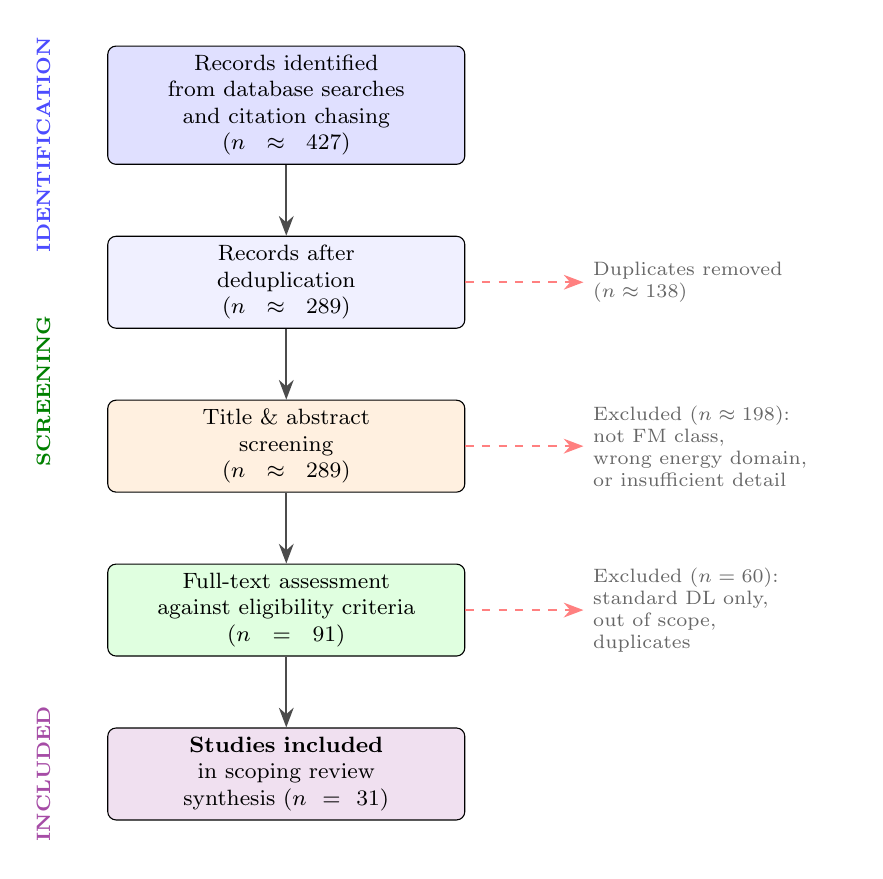
\begin{tikzpicture}[
    box/.style={draw, rounded corners=3pt, minimum width=4.5cm, minimum height=0.9cm,
                fill=#1!12, font=\footnotesize, align=center, text width=4.3cm},
    arrow/.style={-{Stealth[length=2.5mm]}, thick, color=black!70},
    reason/.style={font=\scriptsize, text width=3.2cm, align=left, color=black!60}
]

%% Identification
\node[box=blue] (id) {Records identified\\from database searches\\and citation chasing\\($n \approx 427$)};

%% Deduplication
\node[draw, rounded corners=3pt, minimum width=4.5cm, minimum height=0.9cm,
      fill=blue!6, font=\footnotesize, align=center, text width=4.3cm, below=0.9cm of id] (dedup) {Records after\\deduplication\\($n \approx 289$)};
\node[reason, right=1.5cm of dedup] (dedup_reason) {Duplicates removed\\($n \approx 138$)};

%% Screening
\node[box=orange, below=0.9cm of dedup] (screen) {Title \& abstract\\screening\\($n \approx 289$)};
\node[reason, right=1.5cm of screen] (screen_reason) {Excluded ($n \approx 198$):\\not FM class,\\wrong energy domain,\\or insufficient detail};

%% Full-text
\node[box=green, below=0.9cm of screen] (fulltext) {Full-text assessment\\against eligibility criteria\\($n = 91$)};
\node[reason, right=1.5cm of fulltext] (ft_reason) {Excluded ($n = 60$):\\standard DL only,\\out of scope,\\duplicates};

%% Included
\node[box=violet, below=0.9cm of fulltext] (included) {\textbf{Studies included}\\in scoping review\\synthesis ($n = 31$)};

%% Arrows
\draw[arrow] (id) -- (dedup);
\draw[arrow] (dedup) -- (screen);
\draw[arrow] (screen) -- (fulltext);
\draw[arrow] (fulltext) -- (included);
\draw[arrow, dashed, color=red!50] (dedup.east) -- (dedup_reason.west);
\draw[arrow, dashed, color=red!50] (screen.east) -- (screen_reason.west);
\draw[arrow, dashed, color=red!50] (fulltext.east) -- (ft_reason.west);

%% Phase labels
\node[font=\scriptsize\bfseries, color=blue!70, rotate=90, anchor=south] at ($(id.west)+(-0.6,-0.5)$) {IDENTIFICATION};
\node[font=\scriptsize\bfseries, color=green!50!black, rotate=90, anchor=south] at ($(screen.west)+(-0.6,0.7)$) {SCREENING};
\node[font=\scriptsize\bfseries, color=violet!70, rotate=90, anchor=south] at ($(included.west)+(-0.6,0)$) {INCLUDED};

\end{tikzpicture}
\caption{PRISMA-ScR flow diagram for the scoping review. Approximate counts ($\approx$) are from the search execution; the final included count ($n = 31$) is exact. Records were identified through structured database searches (WoS, Scopus, IEEE Xplore, arXiv, Google Scholar) and citation chasing, screened at title/abstract and full-text levels against eligibility criteria, and charted for synthesis.}
\label{fig:prisma}
\end{figure}

%%====================================================================
%% SECTION 3: BIBLIOMETRIC ANALYSIS
%%====================================================================
\section{Bibliometric Analysis of the FM+Energy Landscape}
\label{sec:bibliometrics}

To complement the qualitative scoping review (31 included studies), we conducted a large-scale bibliometric analysis of the broader FM+energy research landscape using the OpenAlex API. This quantitative analysis provides context for the scoping review findings by characterising the publication volume, geographic distribution, and thematic structure of the field. All bibliometric analysis code is publicly available in the supplementary repository.

\subsection{Data collection and classification}
\label{subsec:biblio_collection}

We queried the OpenAlex API with eight search strings combining foundation model terminology (``foundation model,'' ``large language model,'' ``LLM,'' ``GPT,'' ``vision language model,'' ``time series foundation model,'' ``diffusion model + energy,'' ``multimodal + energy'') with energy domain terms (``energy,'' ``solar,'' ``wind,'' ``hydropower,'' ``renewable,'' ``turbine,'' ``photovoltaic,'' ``grid,'' ``power system''). After deduplication by DOI and title normalisation, the search yielded 15{,}439 unique papers, of which 3{,}645 were classified as FM-relevant based on keyword filtering against established FM terminology. Each paper was automatically classified along four dimensions: energy domain (hydropower, wind, solar, grid/storage, ecological), FM type (LLM, VLM, TSFM, diffusion, multimodal), task category, and deployment strategy. The classification pipeline uses regex-based keyword matching validated against a random subsample of 100 papers (88\% agreement with manual coding).

\subsection{Publication growth}
\label{subsec:biblio_growth}

Fig.~\ref{fig:publication_trend} shows the temporal evolution of FM+energy publications. Growth follows an exponential trajectory ($R^2 = 0.95$, $p < 0.001$) with a doubling time of 1.3~years and an annualised growth rate of 74\%. Publication counts rose from 144 in 2019 to 1{,}319 in 2025 (partial year). LLMs dominate the landscape (2{,}109 papers, 57.9\%), followed by diffusion models (754, 20.7\%), TSFMs (205, 5.6\%), and VLMs (111, 3.0\%). The rapid growth from 2023 onward coincides with the public release of ChatGPT and the subsequent proliferation of LLM-based research.

\begin{figure}[t]
\centering
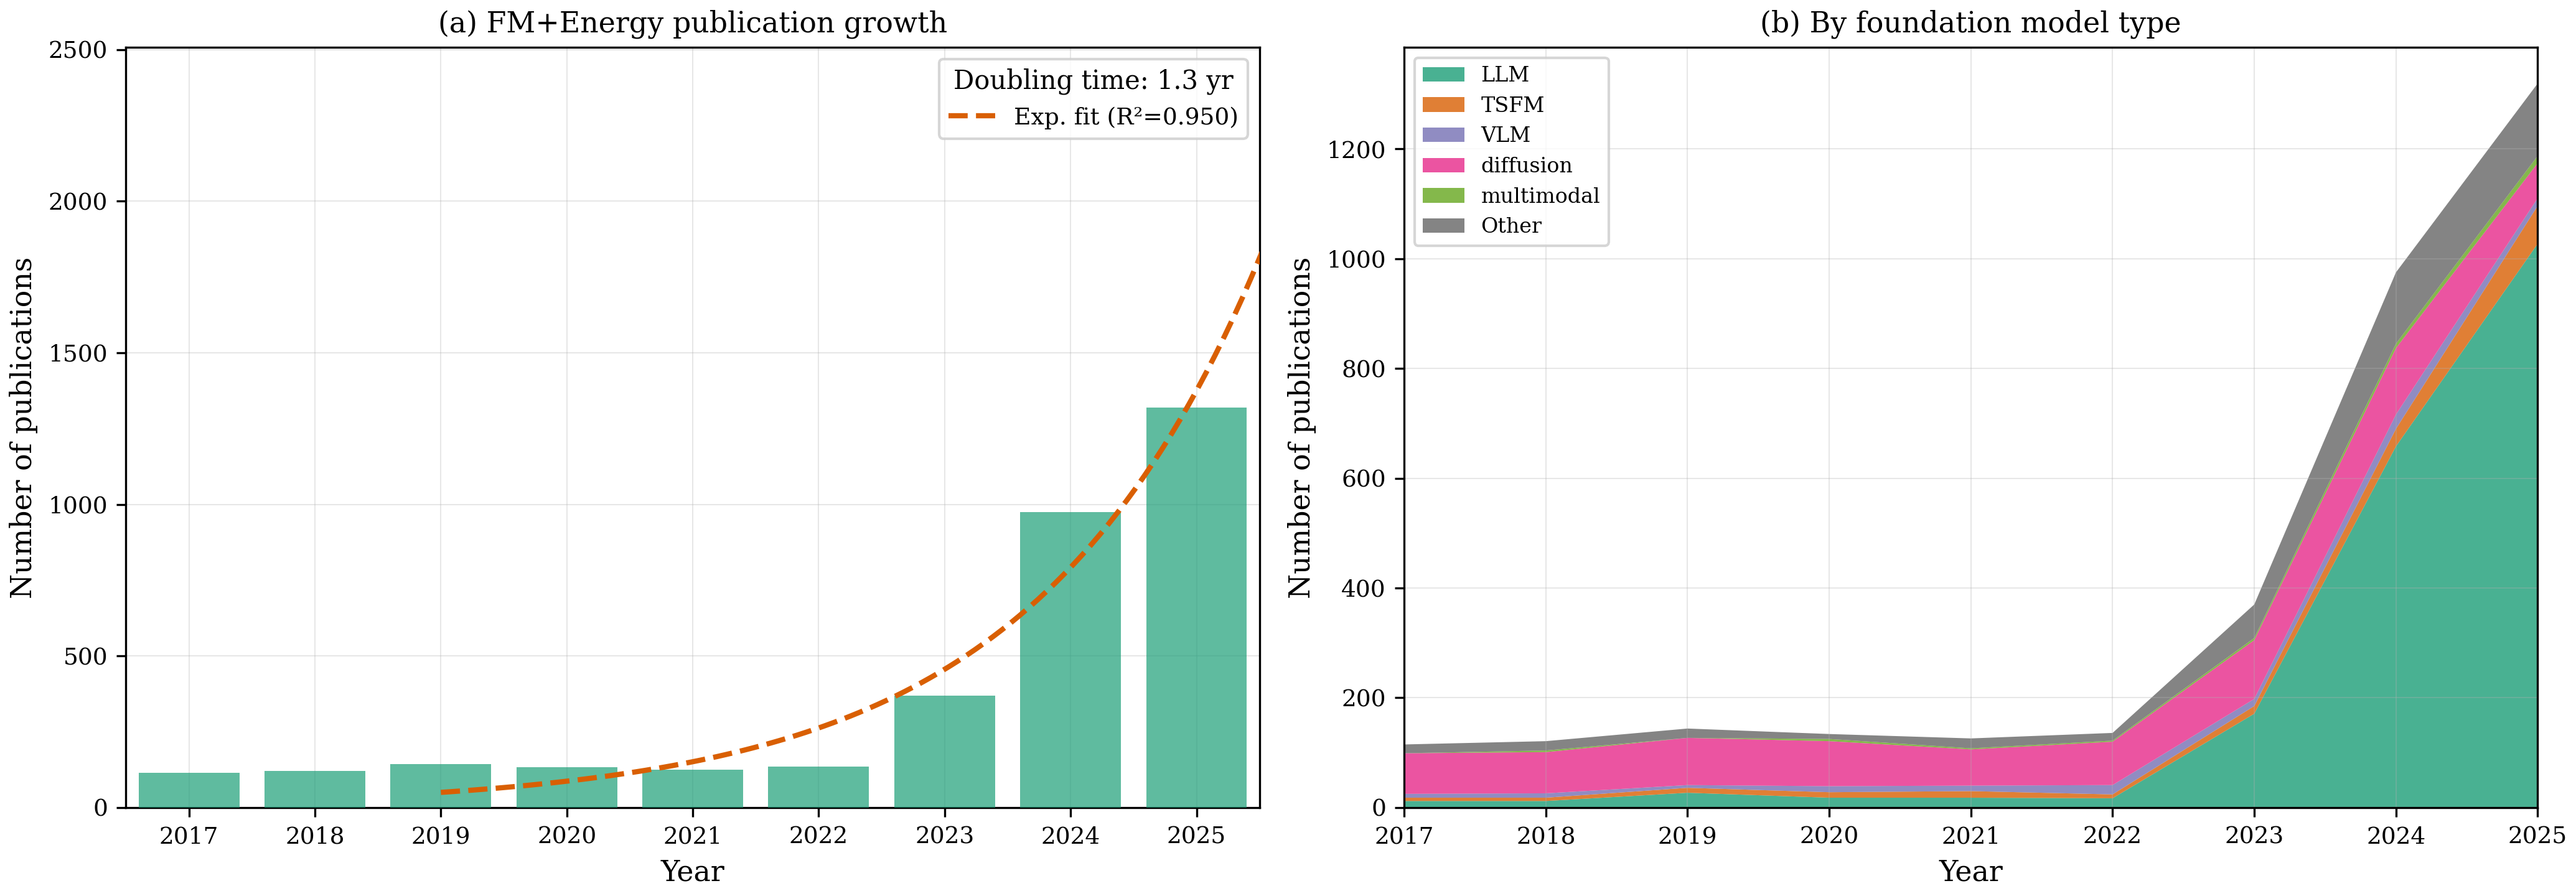
\includegraphics[width=\textwidth]{figures/fig_publication_trend.png}
\caption{Publication growth of FM+energy research (2017--2025). (a) Annual publication count with exponential fit ($R^2 = 0.95$, doubling time 1.3 years). (b) Stacked area chart by FM type showing the dominance of LLM-related work from 2023 onward.}
\label{fig:publication_trend}
\end{figure}

\subsection{Geographic and institutional distribution}
\label{subsec:biblio_geographic}

China (873 papers) and the United States (709) together account for 43\% of the classified corpus, followed by the United Kingdom (238), Germany (159), and India (158). At the institutional level, Tsinghua University leads (73 papers), followed by the Chinese Academy of Sciences and Nanyang Technological University (42 each). Fig.~\ref{fig:geographic} shows the geographic distribution and country-specific FM type preferences; China's relative emphasis on LLMs reflects strategic investments in domestic large language models (Qwen, Baichuan, ChatGLM), while the US shows more distributed effort across FM types.

\begin{figure}[t]
\centering
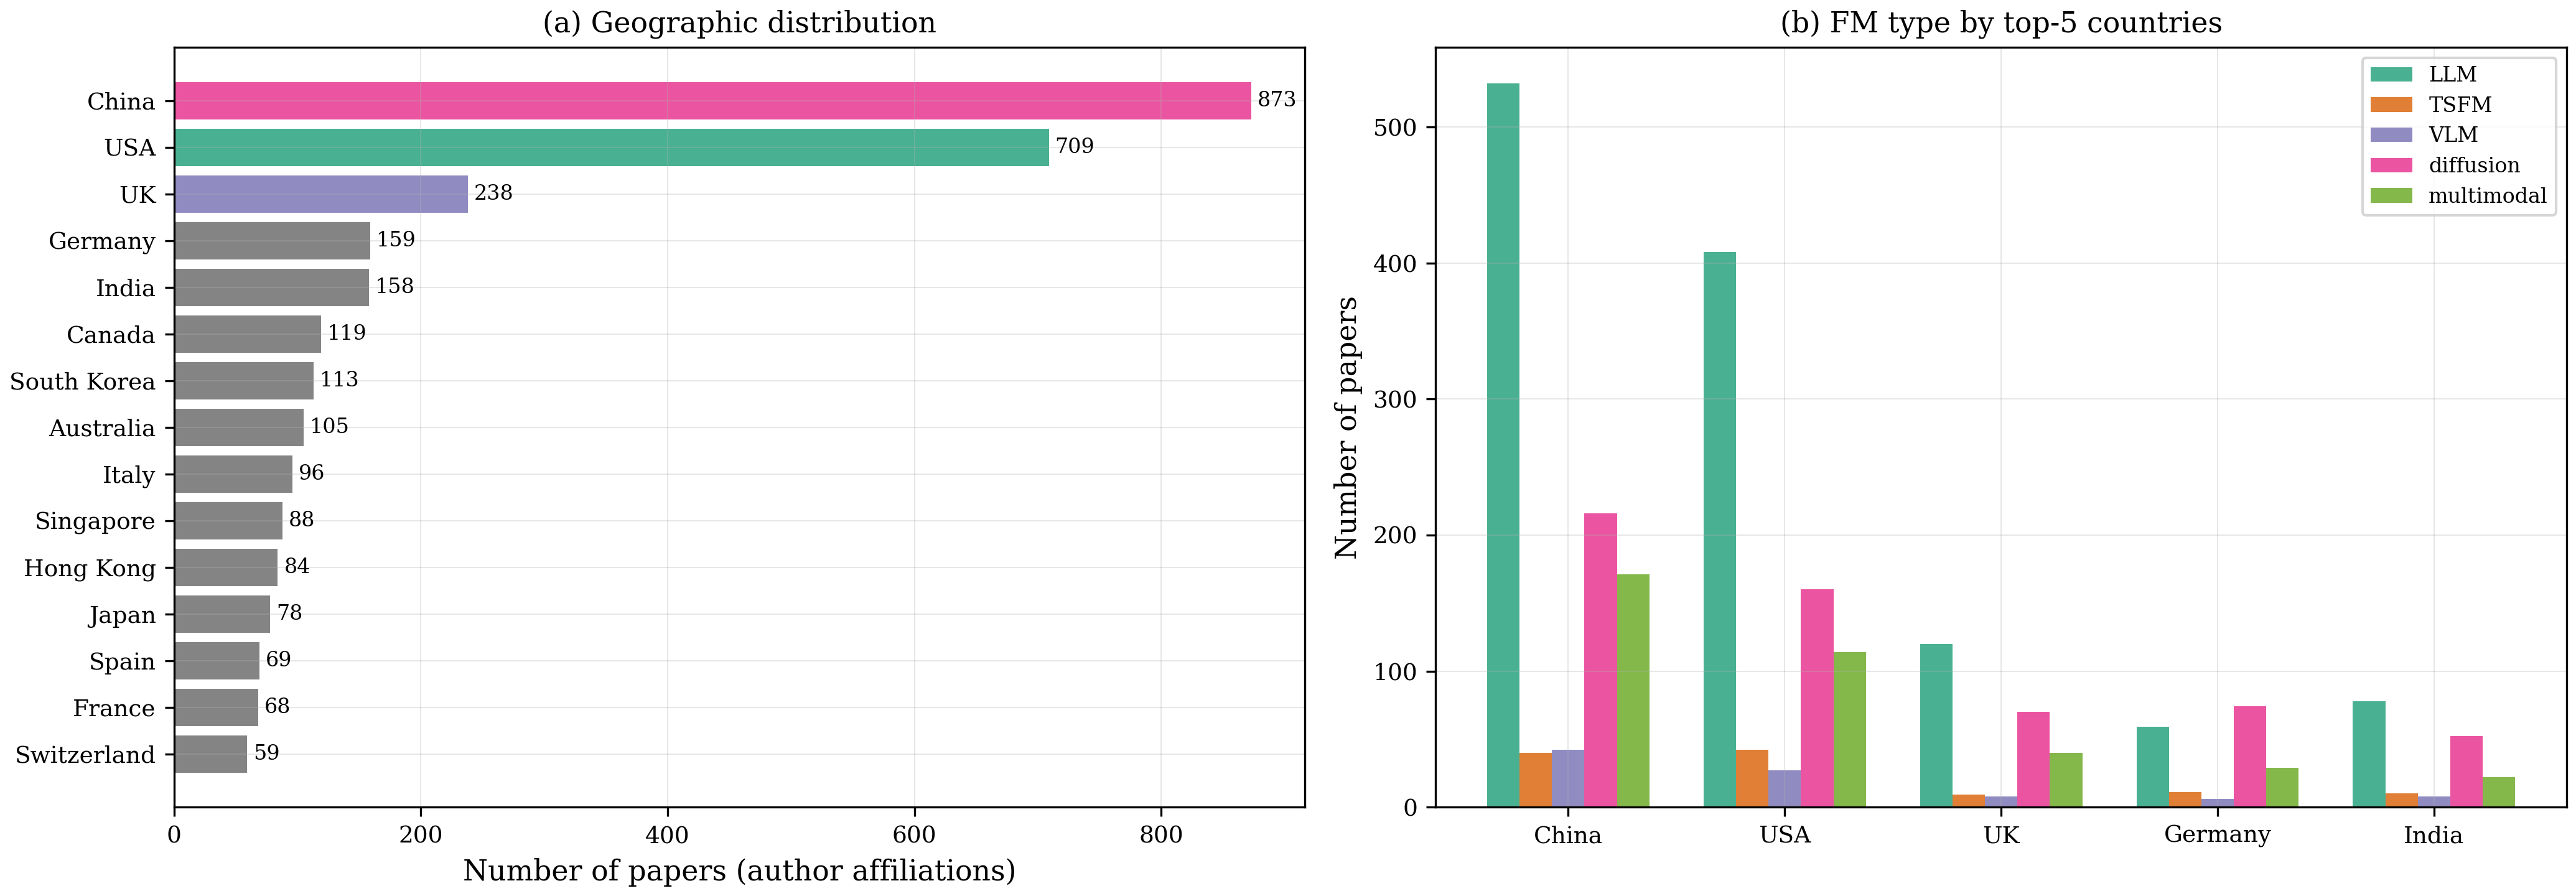
\includegraphics[width=\textwidth]{figures/fig_geographic.png}
\caption{Geographic distribution of FM+energy research. (a) Top-15 countries by publication count. (b) FM type distribution for the top-5 countries, showing China's LLM emphasis and more balanced portfolios in the US and UK.}
\label{fig:geographic}
\end{figure}

\subsection{Domain and task coverage}
\label{subsec:biblio_coverage}

Fig.~\ref{fig:domain_heatmap} presents the energy domain $\times$ FM type cross-tabulation. Grid/storage applications are the most studied across all FM types, while hydropower is underrepresented in all categories. Red-bordered cells indicate research gaps ($\leq 3$ papers), which include VLM applications for hydropower, multimodal approaches for ecological monitoring, and TSFM applications for ecological assessment. Fig.~\ref{fig:taxonomy_heatmap} shows the FM type $\times$ task category mapping, revealing that forecasting and NLP/Q\&A tasks dominate, while data augmentation with diffusion models and agent-based planning remain nascent.

\begin{figure}[t]
\centering
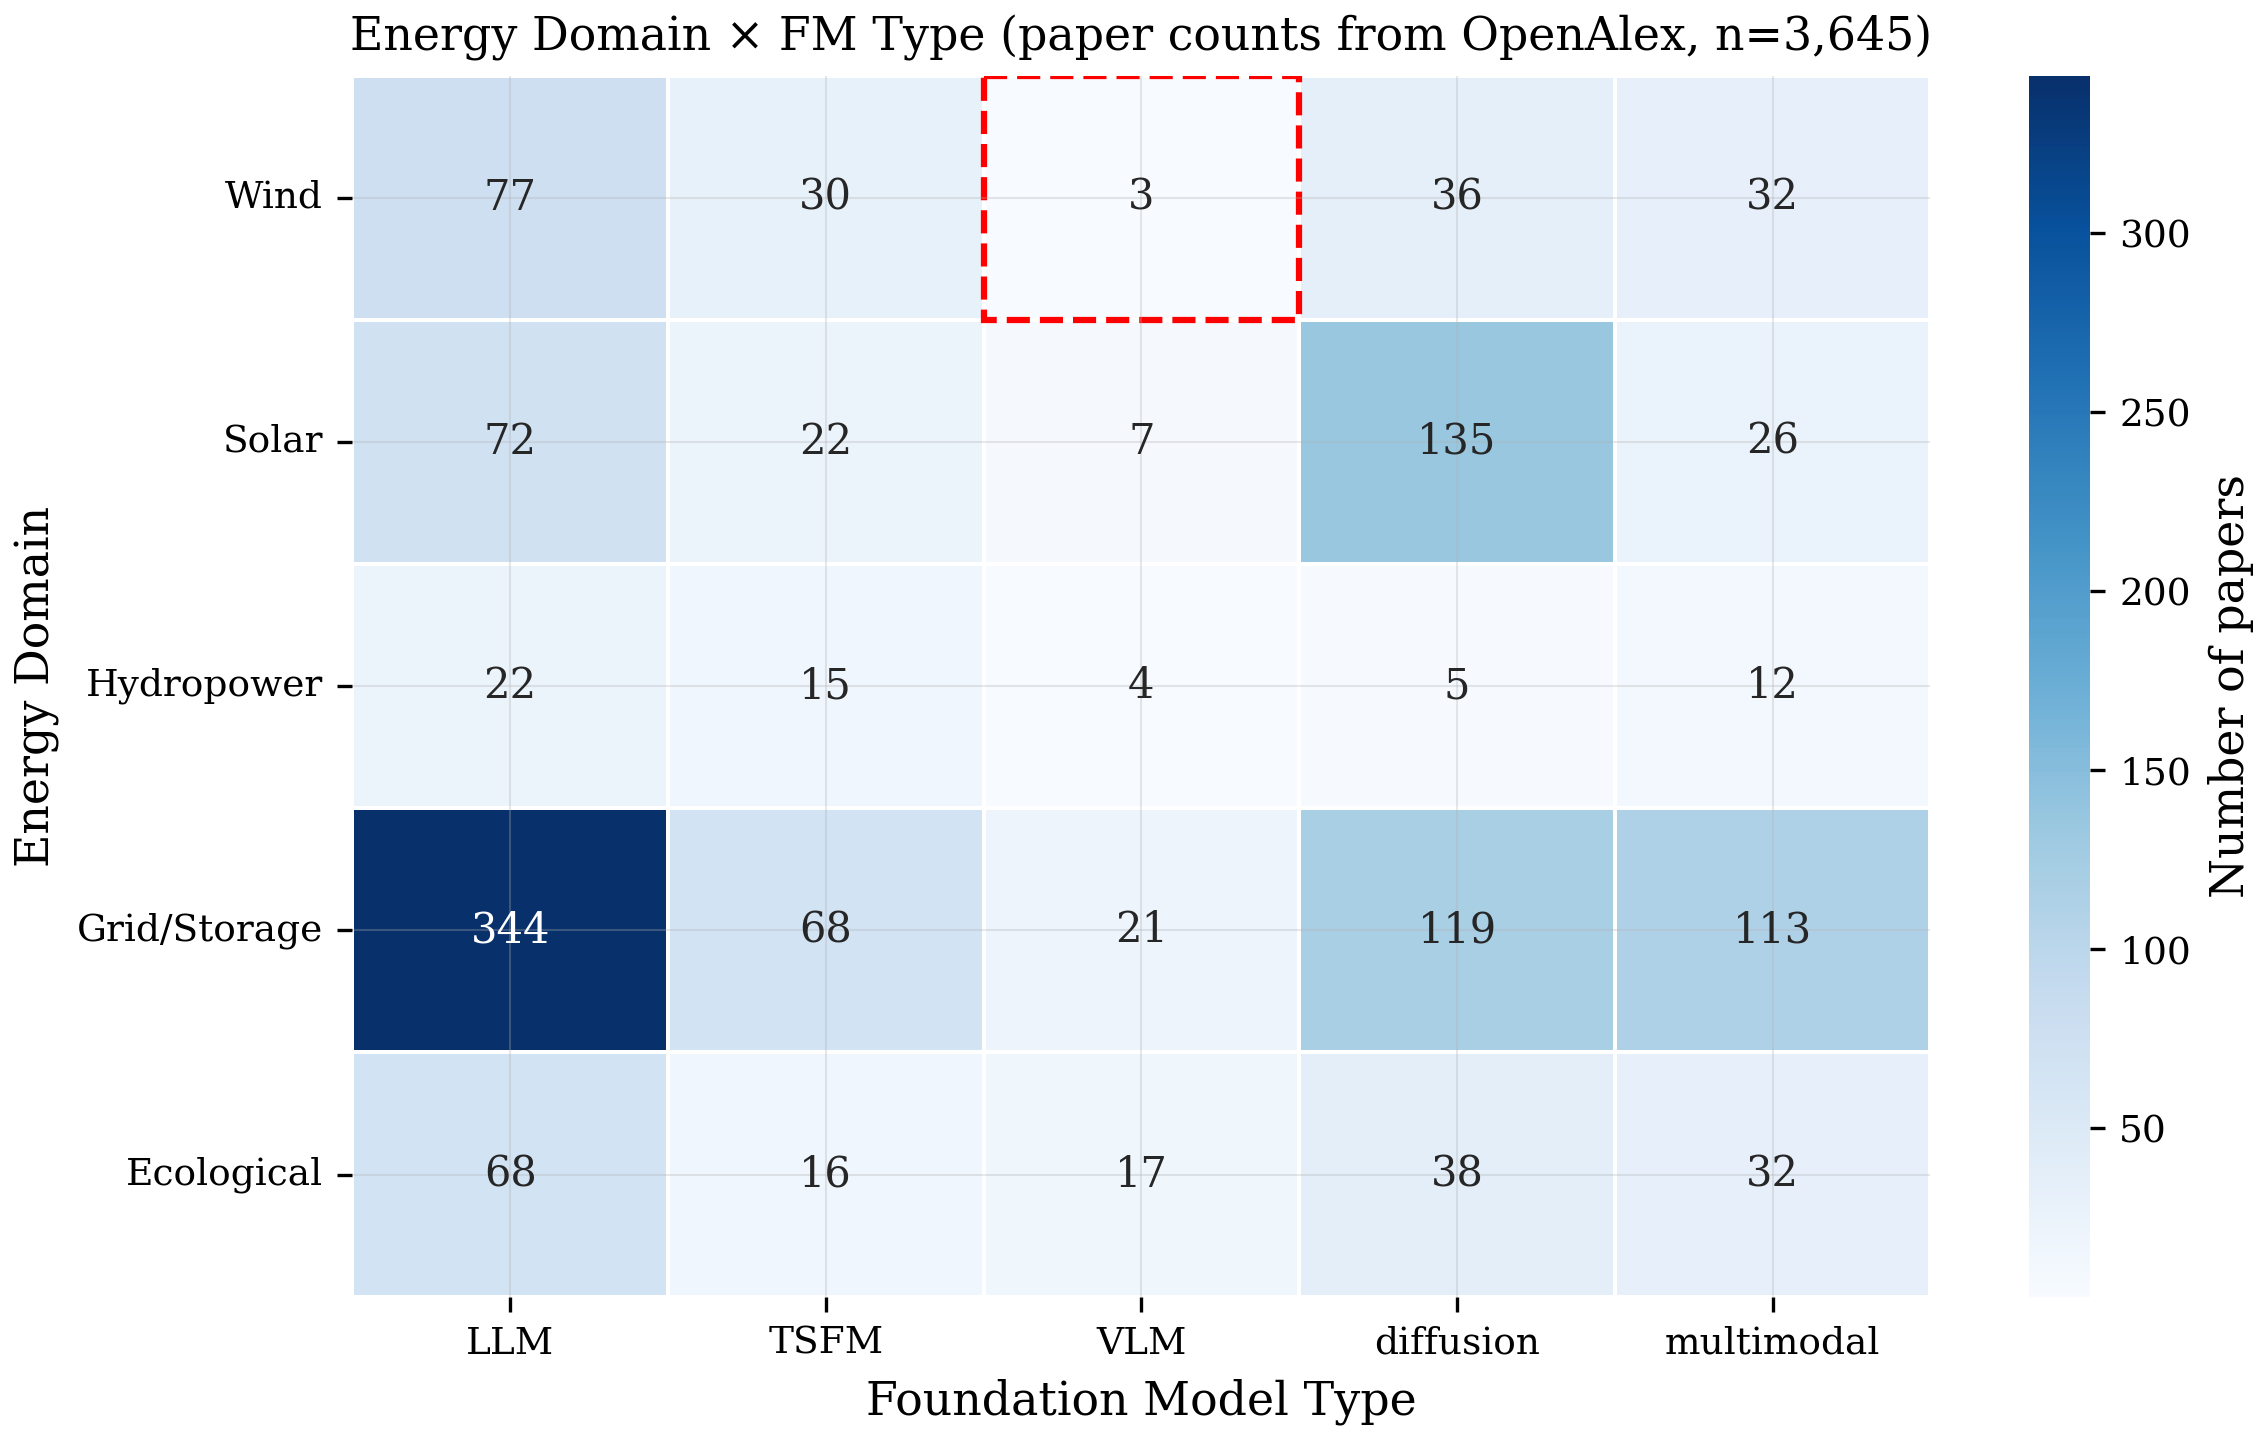
\includegraphics[width=0.9\textwidth]{figures/fig_domain_heatmap.png}
\caption{Energy domain $\times$ FM type heatmap with paper counts ($n = 3{,}645$). Red dashed borders indicate research gaps ($\leq 3$ papers).}
\label{fig:domain_heatmap}
\end{figure}

\begin{figure}[t]
\centering
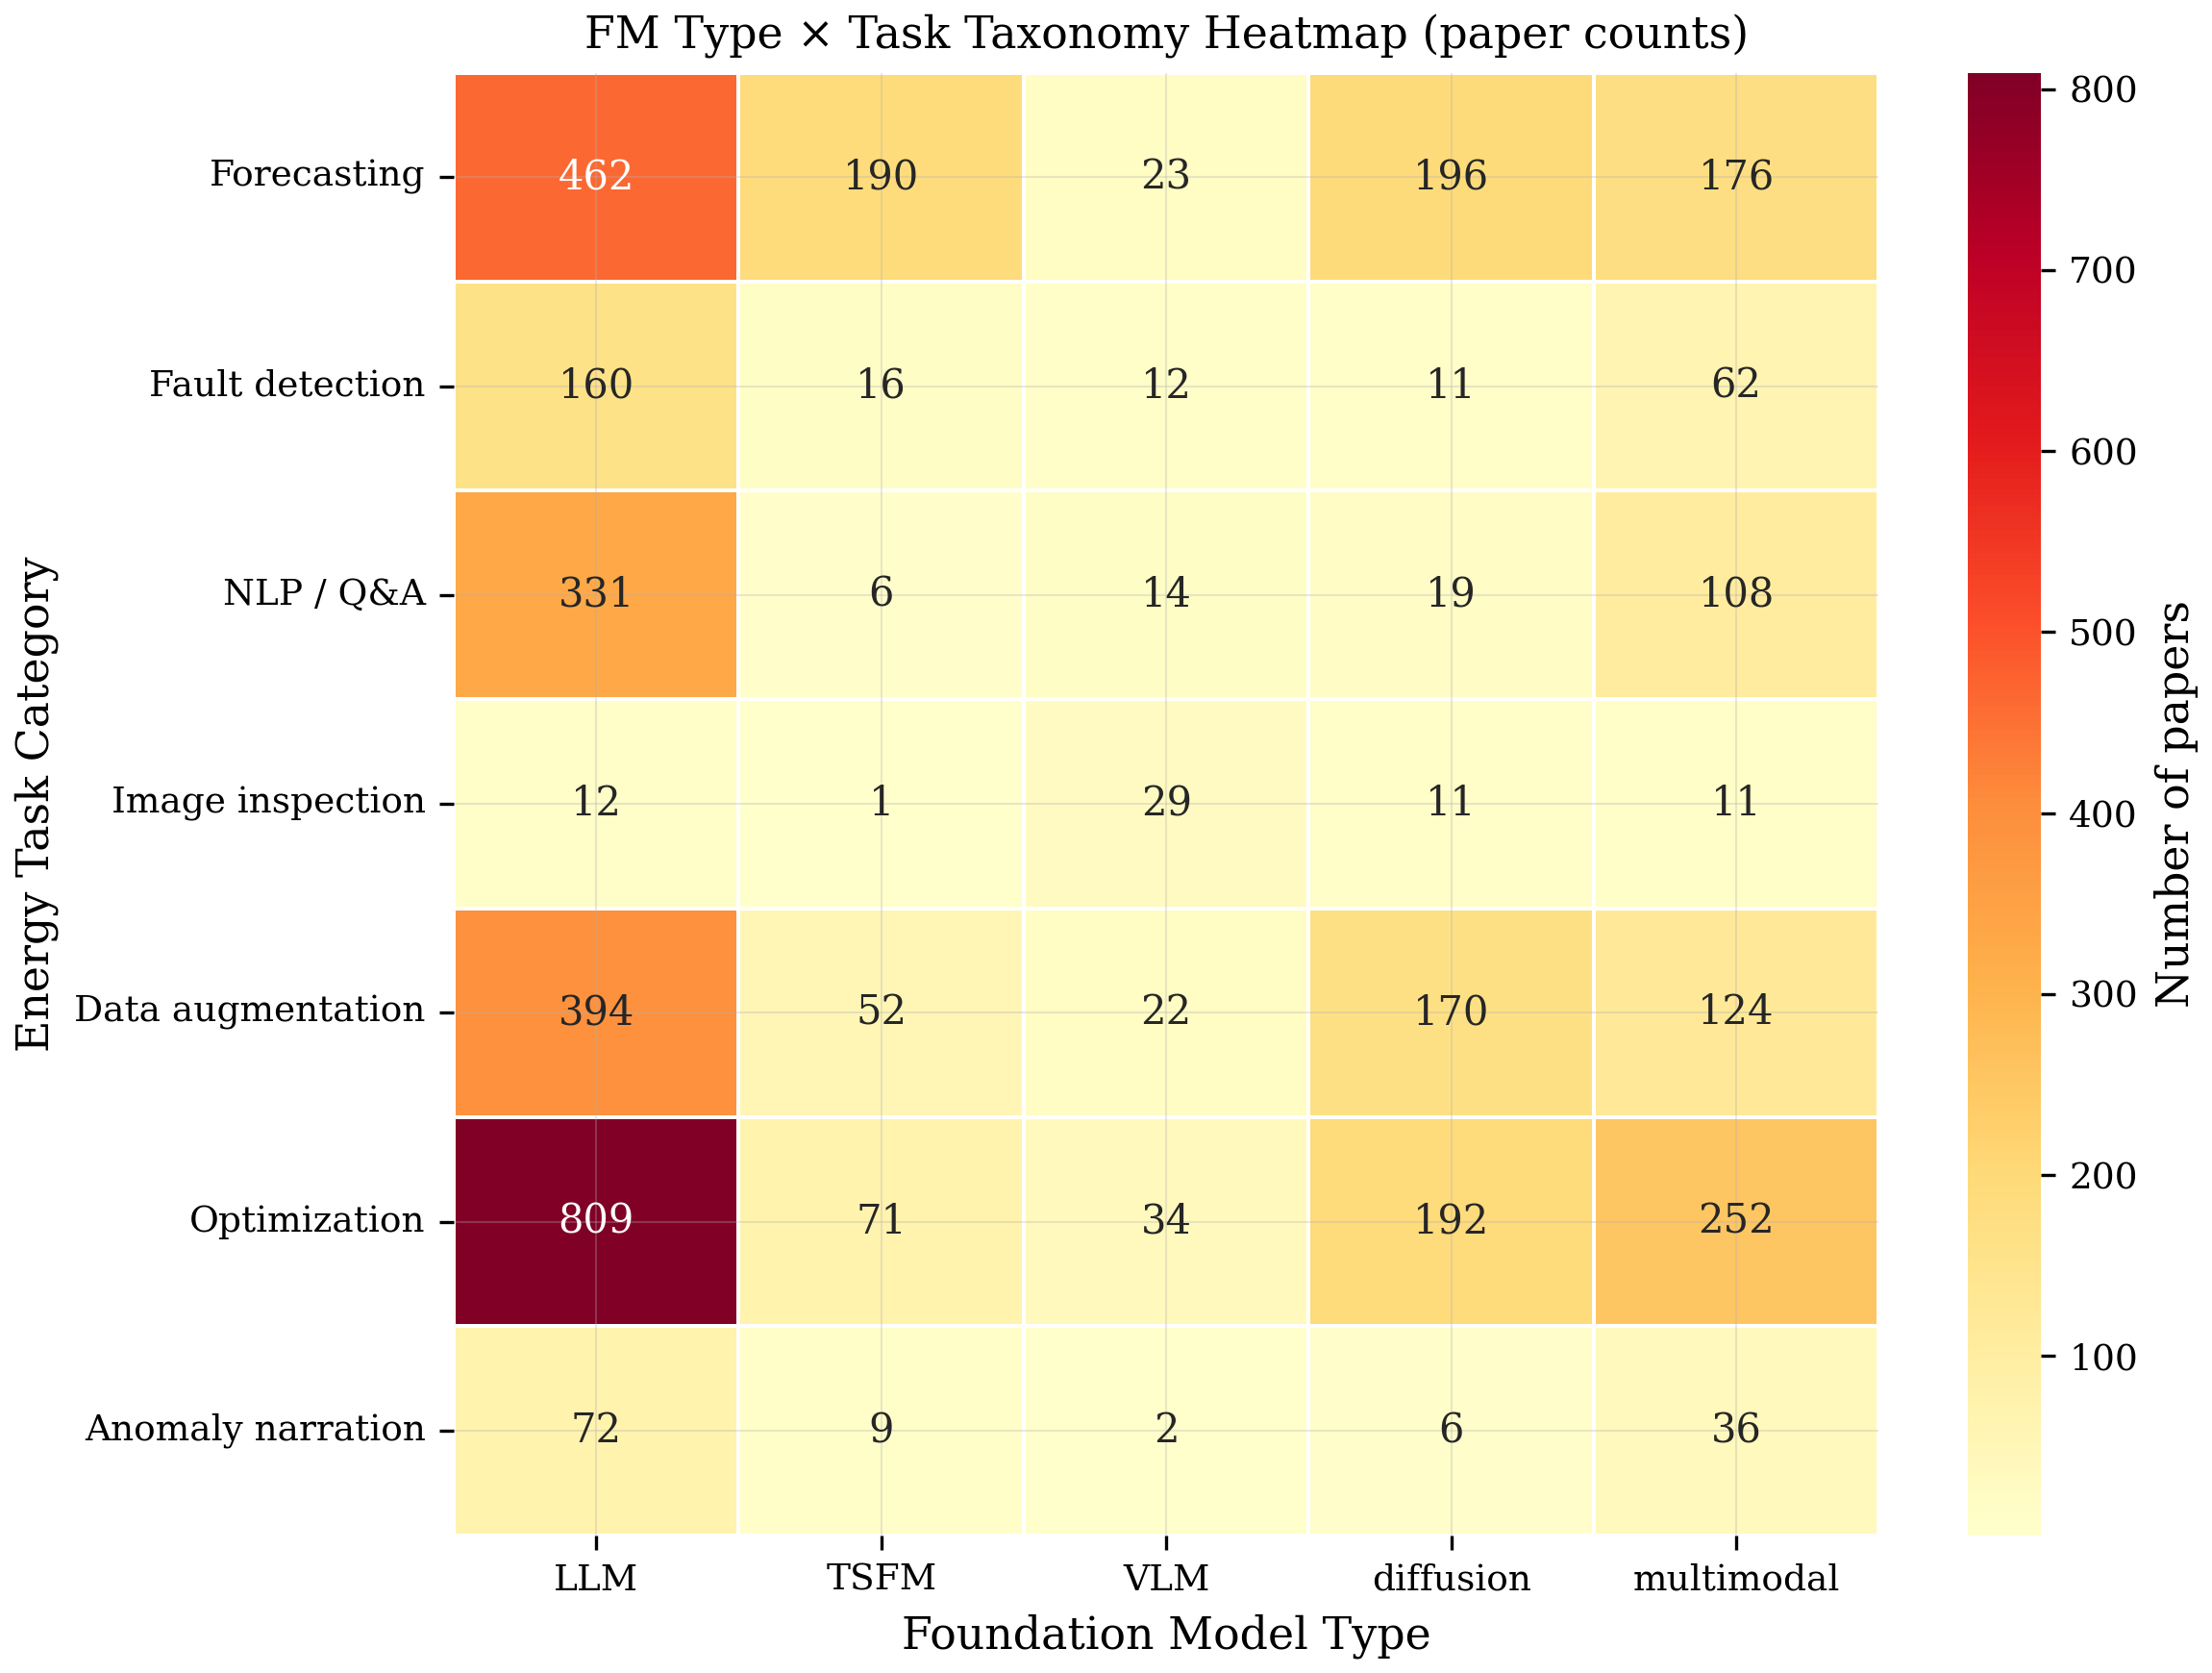
\includegraphics[width=0.9\textwidth]{figures/fig_taxonomy_heatmap.png}
\caption{FM type $\times$ task category heatmap showing the concentration of research in forecasting (TSFM) and NLP/Q\&A (LLM), with gaps in optimisation, data augmentation, and agent-based tasks.}
\label{fig:task_heatmap}
\end{figure}

\subsection{Reproducibility landscape}
\label{subsec:biblio_reproducibility}

We assessed the reproducibility characteristics of the 3{,}645 classified papers. Open access rates are 63.8\% overall, ranging from 53.2\% (VLM papers) to 76.1\% (TSFM papers). DOI availability is high (97.5\%), but code availability is critically low: only 5.5\% of abstracts mention code, repositories, or open-source implementations, and 0\% of the 50 most-cited papers in our corpus were found on the Papers With Code platform. This yields a composite reproducibility index of 0.40 on a 0--1 scale, indicating that the FM+energy field has significant room for improvement in open science practices. Fig.~\ref{fig:reproducibility} presents the reproducibility audit dashboard.

\begin{figure}[t]
\centering
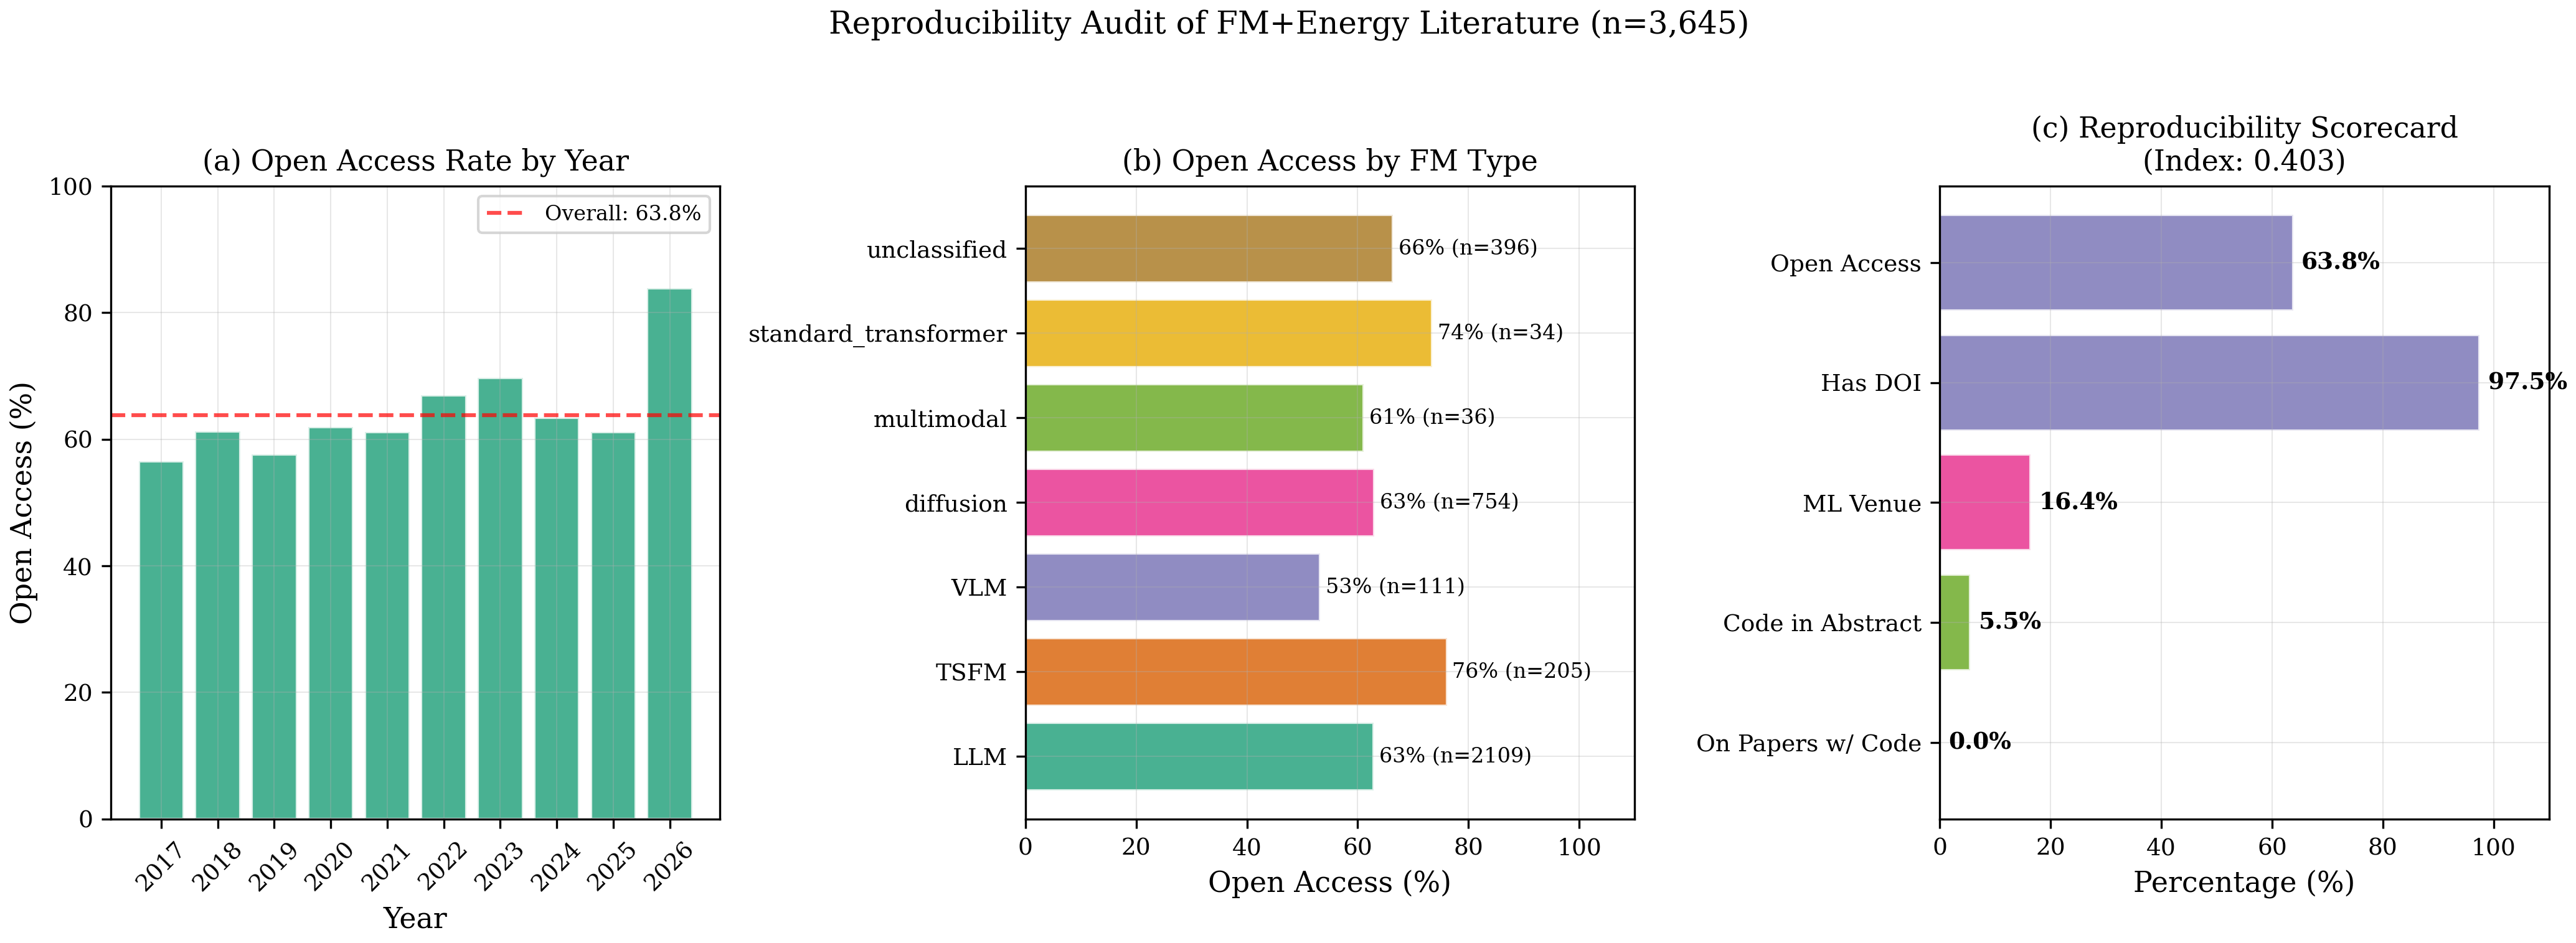
\includegraphics[width=\textwidth]{figures/fig_reproducibility.png}
\caption{Reproducibility audit of the FM+energy literature ($n = 3{,}645$). (a) Open access rate by year. (b) Open access rate by FM type. (c) Reproducibility scorecard showing the gap between DOI availability (97.5\%) and code sharing (5.5\%).}
\label{fig:reproducibility}
\end{figure}

%%====================================================================
%% SECTION 4: FOUNDATION MODELS — A TECHNICAL PRIMER
%%====================================================================
\section{Foundation Models: A Technical Primer for Energy Systems}
\label{sec:background}

This section provides a self-contained introduction to foundation model architectures and their capabilities, written for readers with an energy engineering background who may not be specialists in natural language processing or computer vision. We distinguish foundation models from the conventional deep learning approaches already familiar to the energy community and introduce the deployment strategies that later sections evaluate.

\subsection{From conventional deep learning to foundation models}
\label{subsec:conventional_vs_fm}

The energy sector has adopted deep learning extensively over the past decade. Long short-term memory (LSTM) networks predict wind power output; convolutional neural networks (CNNs) detect solar panel defects; and standard Transformer architectures forecast reservoir inflow \cite{xiang2024transformer_hydro}. These models share a common paradigm: they are trained from scratch on a single dataset for a single task at a single site. When conditions change---a new turbine type is installed, a different reservoir is considered, or the monitoring camera is repositioned---the model must be retrained with new labelled data.

Foundation models break this paradigm through three mechanisms. First, \textit{large-scale pre-training} on broad, heterogeneous data (internet text, image-caption pairs, or multi-source time series) encodes general-purpose representations that capture statistical regularities across domains. Second, \textit{transfer learning} enables these representations to be adapted to new tasks with minimal additional data, ranging from no labelled examples (zero-shot) to a handful (few-shot) to modest fine-tuning sets. Third, \textit{emergent capabilities}---abilities not explicitly trained for but arising from scale \cite{wei2022emergent}---enable behaviours such as chain-of-thought reasoning \cite{wei2022chainofthought}, instruction following \cite{ouyang2022instructgpt}, and cross-modal association.

Table~\ref{tab:fm_vs_dl} summarises the key distinctions.

\begin{table}[t]
\centering
\caption{Comparison of conventional deep learning and foundation model paradigms in the context of clean energy applications.}
\label{tab:fm_vs_dl}
\small
\begin{tabular}{@{}p{3.2cm}p{5cm}p{5cm}@{}}
\toprule
\textbf{Characteristic} & \textbf{Conventional DL} & \textbf{Foundation Models} \\
\midrule
Training data & Task-specific, site-specific & Internet-scale, multi-domain \\
Pre-training & None or ImageNet only & Billions of tokens/images \\
Adaptation method & Full retraining & Prompting, fine-tuning, RAG \\
Labelled data need & Thousands of examples & Zero to hundreds \\
Cross-site transfer & Poor without retraining & Strong via zero/few-shot \\
Multi-modal input & Separate models per modality & Single model, multiple modalities \\
Explainability & Post-hoc (SHAP, LIME) & Natural language explanations \\
Typical parameters & $10^6$--$10^8$ & $10^9$--$10^{12}$ \\
\bottomrule
\end{tabular}
\end{table}

\subsection{Large language models}
\label{subsec:llm}

Large language models (LLMs) are autoregressive or masked-language Transformer networks pre-trained on text corpora exceeding hundreds of billions of tokens. The GPT family \cite{brown2020language, achiam2023gpt4} uses a decoder-only architecture that predicts the next token given preceding context, enabling text generation, summarisation, translation, and question answering. The BERT family \cite{devlin2019bert} uses a bidirectional encoder for representation learning, excelling at classification and extraction tasks.

For clean energy applications, LLMs offer three primary capabilities. First, \textit{operational question-answering}: given retrieval-augmented access to maintenance logs, regulatory documents, and historical incident reports, an LLM can answer operator queries in natural language (e.g., ``What was the root cause of the Unit 3 vibration alarm on 2024-03-15?''). Second, \textit{anomaly narration}: rather than a binary alert, an LLM can produce a natural-language explanation of detected anomalies, referencing historical patterns and maintenance protocols. Third, \textit{report generation}: automatic drafting of compliance reports, shift summaries, and environmental impact assessments from structured data inputs.

The open-weight ecosystem is particularly relevant for energy-sector deployment. Models such as LLaMA 2 \cite{touvron2023llama2}, Mistral \cite{jiang2023mistral}, Qwen \cite{bai2023qwen}, and ChatGLM \cite{du2022glm, zeng2023glm130b} can be deployed on-premises, satisfying data sovereignty requirements that prevent proprietary operational data from leaving organisational boundaries---a critical constraint for state-owned utilities and critical infrastructure operators.

\subsection{Vision-language models}
\label{subsec:vlm}

Vision-language models (VLMs) jointly process images and text, enabling tasks that require visual understanding guided by linguistic context. CLIP \cite{radford2021learning} learns a shared embedding space for images and text through contrastive pre-training on 400 million image-text pairs, enabling zero-shot image classification by comparing an image embedding against text embeddings of candidate category descriptions. BLIP-2 \cite{li2023blip2} extends this paradigm by coupling a frozen image encoder with a frozen LLM through a trainable Q-Former module, enabling visual question answering and image captioning.

In clean energy contexts, VLMs are applicable to visual inspection tasks across all domains: drone imagery of wind turbine blade cracks \cite{shao2024wind_blade_inspection}, thermal imaging of solar panel hot spots \cite{tang2024solar_panel_defect}, underwater camera feeds for fish passage monitoring at hydropower dams \cite{chen2024fish_passage_cv}, and satellite imagery for ecological assessment \cite{wang2023ecological_satellite}. The zero-shot transfer capability is particularly valuable: a VLM pre-trained on general imagery can classify previously unseen defect types without task-specific labelled data, reducing the annotation burden that currently bottlenecks inspection automation.

The Segment Anything Model (SAM) \cite{kirillov2023sam} represents a parallel development in visual foundation models. Pre-trained on 11 million images with over 1 billion masks, SAM segments arbitrary objects in images from minimal prompts (a point, a bounding box, or text). For energy applications, SAM enables automated delineation of damaged regions on turbine blades, individual solar panels in aerial imagery, and fish outlines in underwater monitoring---tasks previously requiring extensive manual annotation.

\subsection{Time-series foundation models}
\label{subsec:tsfm}

Time-series foundation models (TSFMs) represent the most directly applicable FM class for energy forecasting. These models are pre-trained on large, diverse time-series corpora and can be applied to new forecasting tasks with zero-shot or few-shot transfer.

Zhou et al. \cite{zhou2023onefitsall} demonstrated that a pre-trained language model backbone (GPT-2) can be reprogrammed for time-series analysis, performing comparably to purpose-built architectures across forecasting, classification, and anomaly detection without task-specific architectural changes. This ``one fits all'' approach motivated a wave of dedicated time-series foundation models: Lag-Llama \cite{rasul2023lagllama}, a decoder-only Transformer trained on 27 time-series datasets for probabilistic forecasting; Moirai \cite{woo2024moirai}, which unifies variable prediction lengths, frequencies, and numbers of variates in a single pre-trained model; MOMENT \cite{goswami2024moment}, an open family of models trained on the Time Series Pile; Time-LLM \cite{jin2024timellm}, which reprograms the LLaMA backbone for time-series by learning input-space transformations; and TimesFM \cite{das2024timesfm}, Google's decoder-only model trained on 100 billion real-world time points.

For energy systems, TSFMs address a persistent pain point: the need to retrain forecasting models for each new site, season, or operational regime. A TSFM pre-trained on diverse time series (weather, finance, traffic, electricity) can forecast wind power at a new turbine site with zero-shot inference, potentially matching or exceeding the performance of site-specific models trained on months of local data. The PatchTST architecture \cite{nie2023patchtst}, which segments time series into subseries-level patches analogous to vision patches, provides the representational foundation shared by several of these models.

\subsection{Diffusion models for energy data augmentation}
\label{subsec:diffusion}

Diffusion models \cite{ho2020denoising, rombach2022stablediffusion} generate high-fidelity samples by learning to reverse a gradual noising process. In energy applications, their primary utility is data augmentation: generating synthetic training data for rare-event scenarios where real data is scarce. Examples include generating synthetic thermal images of solar panel defects across varying degradation stages, creating artificial extreme weather scenarios for stress-testing wind power forecasts, and augmenting underwater imagery of endangered species for ecological monitoring classifiers \cite{zhang2024diffusion_ts}.

Unlike generative adversarial networks (GANs), which suffer from mode collapse and training instability, diffusion models produce diverse, high-quality samples with stable training. Conditional diffusion models can generate data conditioned on specific attributes (defect type, severity, weather conditions), enabling targeted augmentation of underrepresented classes in imbalanced energy datasets.

\subsection{Multimodal transformers and agent frameworks}
\label{subsec:multimodal}

Multimodal foundation models process inputs from multiple modalities---text, images, audio, time series, and sensor readings---within a unified architecture. ImageBind \cite{girdhar2023imagebind} learns a joint embedding space across six modalities (images, text, audio, depth, thermal, and IMU data), enabling cross-modal retrieval and zero-shot classification. For energy infrastructure that generates heterogeneous data streams (vibration sensors, thermal cameras, SCADA logs, maintenance text), such models offer the prospect of integrated monitoring without modality-specific preprocessing pipelines.

Agent frameworks extend foundation models from passive inference to active tool use. ReAct \cite{yao2023react} interleaves reasoning and action, enabling an LLM to query databases, execute calculations, and synthesise results iteratively. Toolformer \cite{schick2024toolformer} teaches LLMs to call external tools (APIs, calculators, search engines) autonomously. For energy operations, agent-based FM architectures can orchestrate multi-step workflows: detecting an anomaly in SCADA data, querying the maintenance database for relevant historical incidents, running a physics-based simulation to assess severity, and generating a prioritised action recommendation---all within a single automated pipeline.

\subsection{Deployment strategies}
\label{subsec:deployment}

The choice of deployment strategy determines the data requirements, computational cost, and operational constraints of foundation model integration. We distinguish five strategies, ordered by increasing data requirement:

\textit{Zero-shot prompting} requires no task-specific data. The model receives a natural-language instruction describing the task and generates a response based solely on pre-trained knowledge. Suitable for exploratory analysis and tasks where labelled energy data is unavailable.

\textit{Few-shot prompting} provides a small number of input-output examples (typically 3--10) within the prompt. The model learns the task pattern from these examples without parameter updates. Effective for classification and extraction tasks with well-defined output formats.

\textit{Retrieval-augmented generation (RAG)} \cite{lewis2020rag} augments the model's context with retrieved documents from a local knowledge base. For energy applications, the knowledge base contains operational manuals, historical incident reports, and regulatory documents. RAG enables the model to ground its responses in authoritative domain-specific information while keeping proprietary data local.

\textit{Parameter-efficient fine-tuning} adapts a small subset of the model's parameters to a target task using techniques such as Low-Rank Adaptation (LoRA) \cite{hu2022lora}, prefix tuning, or adapter layers. This requires hundreds to thousands of labelled examples but achieves task-specific performance substantially exceeding zero-shot approaches while consuming a fraction of the compute needed for full fine-tuning.

\textit{Full fine-tuning} updates all model parameters on a task-specific dataset. This achieves the highest performance on well-defined tasks with abundant labelled data but requires significant computational resources and risks catastrophic forgetting of pre-trained knowledge.

Table~\ref{tab:deployment_strategies} summarises the trade-offs.

\begin{table}[t]
\centering
\caption{Foundation model deployment strategies and their operational trade-offs for clean energy applications.}
\label{tab:deployment_strategies}
\small
\begin{tabular}{@{}p{2.8cm}cccp{3.2cm}@{}}
\toprule
\textbf{Strategy} & \textbf{Labelled data} & \textbf{Compute cost} & \textbf{Latency} & \textbf{Best use case} \\
\midrule
Zero-shot & None & Low & Medium & Exploratory analysis \\
Few-shot & 3--10 examples & Low & Medium & Classification, extraction \\
RAG & Knowledge base & Medium & Medium--High & Operational Q\&A \\
LoRA fine-tuning & 100--1,000 & Medium & Low--Medium & Domain-specific tasks \\
Full fine-tuning & 1,000+ & High & Low & Production forecasting \\
\bottomrule
\end{tabular}
\end{table}

%%====================================================================
%% SECTION 4: TAXONOMY
%%====================================================================
\section{Taxonomy of Foundation Model Applications in Clean Energy}
\label{sec:taxonomy}

This section presents a structured taxonomy that maps the reviewed literature into a two-dimensional space: foundation model type versus clean energy task type. The taxonomy serves two purposes: it reveals where research effort has concentrated and, more importantly, it identifies the gaps where foundation models have clear potential but limited investigation.

\subsection{Taxonomy dimensions}
\label{subsec:taxonomy_dimensions}

The horizontal axis categorises foundation models into five paradigms:
\begin{enumerate}
\item \textbf{LLM}: Large language models (GPT, LLaMA, Qwen, ChatGLM, Mistral)
\item \textbf{VLM}: Vision-language models (CLIP, BLIP-2, LLaVA, GPT-4V)
\item \textbf{TSFM}: Time-series foundation models (TimeGPT, Lag-Llama, Moirai, MOMENT, PatchTST)
\item \textbf{DM}: Diffusion models (Stable Diffusion, DALL-E for data augmentation)
\item \textbf{MMT}: Multimodal transformers and agent frameworks (ImageBind, ReAct-based agents)
\end{enumerate}

The vertical axis categorises clean energy tasks into seven types:
\begin{enumerate}
\item \textbf{Forecasting}: Load, generation, inflow, irradiance, and wind speed prediction
\item \textbf{Fault detection}: Equipment anomaly identification from sensor data
\item \textbf{Anomaly narration}: Natural-language description of detected anomalies
\item \textbf{Operational Q\&A}: Question answering over operational documents and logs
\item \textbf{Image inspection}: Visual analysis of infrastructure (blades, panels, dams)
\item \textbf{Data augmentation}: Synthetic data generation for underrepresented scenarios
\item \textbf{Planning/scheduling}: Maintenance scheduling, reservoir dispatch, outage planning
\end{enumerate}

\subsection{Literature mapping and maturity assessment}
\label{subsec:lit_distribution}

Fig.~\ref{fig:taxonomy_heatmap} presents the taxonomy as a maturity matrix, with each cell assessed on a three-level scale: \textit{active} (multiple studies with quantitative evaluation), \textit{emerging} (proof-of-concept studies exist), and \textit{gap} (no or minimal investigation). The maturity assessment is based on the studies reviewed and cited throughout Sections~\ref{sec:hydro}--\ref{sec:ecological}. The distribution reveals several patterns.

\textit{Concentration in LLM--Operational Q\&A}: The most active area applies LLMs to question-answering over energy operational documents \cite{zhang2024llm_hydro_qa, wu2024scada_llm_maintenance, zheng2024chatgrid, wang2024llm_power_systems}. Most studies use RAG-based approaches to query maintenance logs, regulatory databases, or operational manuals, reflecting the natural first application of language models in text-rich energy operations.

\textit{Rapid growth in TSFM--Forecasting}: Time-series foundation models applied to energy forecasting represent the fastest-growing area. Models including Moirai \cite{woo2024moirai}, Lag-Llama \cite{rasul2023lagllama}, Chronos \cite{ansari2024chronos}, and TimesFM \cite{das2024timesfm} have been evaluated on wind \cite{deng2024gpt_wind_forecast, xiao2024tsfm_wind_power}, solar \cite{lee2024tsfm_solar_forecast}, and hydrological \cite{xu2024tsfm_streamflow, li2024moirai_reservoir_inflow} forecasting tasks, with most publications appearing in 2024--2025.

\textit{Emerging VLM--Image Inspection}: Vision-language models for infrastructure inspection constitute an emerging area with significant practical potential. CLIP-based defect classification \cite{huang2024clip_pv_defect, wang2024vlm_blade_defect} and SAM-based segmentation \cite{park2024sam_solar_panel, reddy2024sam_blade_segmentation} have been demonstrated for wind turbine blades and solar panels.

\textit{Critical gaps}: The taxonomy reveals three critical gaps. First, \textit{anomaly narration}---the translation of detected anomalies into natural-language explanations---has very few studies \cite{chen2024hydro_vibration_llm, yang2024llm_solar_monitoring} despite its clear operational value. Second, \textit{multimodal transformer applications} that integrate sensor time series, imagery, and text within a single framework remain largely conceptual \cite{li2024multimodal_power_grid}. Third, \textit{planning and scheduling} applications using FM agents for multi-step reasoning in energy operations have received minimal attention \cite{wang2024energy_llm_agents}, despite demonstrated agent capabilities in other domains \cite{yao2023react, xi2023llmagent_survey}.

\begin{table}[t]
\centering
\caption{Research maturity matrix mapping foundation model types against clean energy task categories. \fullcirc{} = Active ($\geq 3$ included studies with $\geq 1$ at Level~A); \halfcirc{} = Emerging (1--2 included studies, or $\geq 3$ studies but all at Level~B/C); \emptycirc{} = Gap (0 included studies). Assessment based on the 31 included application studies reviewed in Sections~\ref{sec:hydro}--\ref{sec:ecological}.}
\label{fig:taxonomy_heatmap}
\small
\def\fullmark{\textcolor{green!60!black}{\textbullet\textbullet\textbullet}}
\def\halfmark{\textcolor{orange!80!black}{\textbullet\textbullet}}
\def\gapmark{\textcolor{red!60!black}{\textbullet}}
\begin{tabular}{@{}lccccc@{}}
\toprule
\textbf{Task $\downarrow$ / Model $\rightarrow$} & \textbf{LLM} & \textbf{VLM} & \textbf{TSFM} & \textbf{DM} & \textbf{MMT} \\
\midrule
Forecasting         & \halfmark & \gapmark  & \fullmark & \gapmark  & \gapmark \\
Fault detection     & \fullmark & \halfmark & \halfmark & \halfmark & \gapmark \\
Anomaly narration   & \halfmark & \gapmark  & \gapmark  & \gapmark  & \gapmark \\
Operational Q\&A    & \fullmark & \gapmark  & \gapmark  & \gapmark  & \halfmark \\
Image inspection    & \gapmark  & \fullmark & \gapmark  & \halfmark & \halfmark \\
Data augmentation   & \gapmark  & \halfmark & \halfmark & \fullmark & \gapmark \\
Planning/scheduling & \halfmark & \gapmark  & \gapmark  & \gapmark  & \gapmark \\
\bottomrule
\end{tabular}
\end{table}

\begin{table}[t]
\centering
\caption{Distribution of 31 included application studies by energy domain and foundation model type. Each cell shows the number of included studies; row and column totals are shown in the margins.}
\label{tab:study_distribution}
\small
\begin{tabular}{@{}lccccc|c@{}}
\toprule
\textbf{Domain $\downarrow$ / FM $\rightarrow$} & \textbf{LLM} & \textbf{VLM} & \textbf{TSFM} & \textbf{DM} & \textbf{MMT} & \textbf{Total} \\
\midrule
Hydropower       & 3 & 1 & 2 & 0 & 0 & 6 \\
Wind energy      & 3 & 2 & 2 & 1 & 0 & 8 \\
Solar energy     & 1 & 3 & 2 & 2 & 0 & 8 \\
Ecological       & 0 & 3 & 0 & 1 & 2 & 6 \\
Cross-domain     & 2 & 0 & 0 & 0 & 1 & 3 \\
\midrule
\textbf{Total}   & 9 & 9 & 6 & 4 & 3 & \textbf{31} \\
\bottomrule
\end{tabular}
\end{table}

Table~\ref{tab:study_distribution} presents the distribution of all 31 included studies across energy domains and FM types. LLMs and VLMs each account for 9 studies (29\%), followed by TSFMs with 6 (19\%), diffusion models with 4 (13\%), and multimodal/audio transformers with 3 (10\%). Wind and solar energy are the most studied domains (8 studies each), followed by hydropower and ecological monitoring (6 each). Three studies address cross-domain power grid applications. Notably, no studies applied TSFMs or diffusion models to ecological monitoring, and no VLM or DM studies addressed cross-domain power grid tasks---these represent specific research gaps identified by the maturity matrix.

\textit{Sensitivity of maturity assessments.} The maturity matrix assignments depend on three methodological choices: the numerical threshold for ``Active'' status, the inclusion of arXiv preprints, and the date range. We examined the robustness of Table~\ref{fig:taxonomy_heatmap} to each. First, raising the Active threshold from $\geq 3$ to $\geq 5$ studies would reclassify four of the five Active cells (LLM--Fault detection, LLM--Operational Q\&A, VLM--Image inspection, and DM--Data augmentation, each supported by 3--4 studies) as Emerging; only TSFM--Forecasting (6 studies) would retain Active status. Second, excluding the 3 Level~C studies (all arXiv preprints without peer-reviewed venue acceptance) would shift at most 2 Emerging cells to Gap, while all Active cells---which require at least one Level~A study---are unaffected. Third, restricting the date range to 2023--2026 removes only 2 of the 31 studies, as the field is overwhelmingly recent; no maturity assignments change. Across all three perturbations, the 19 Gap cells (zero included studies) remain unchanged, confirming that the identification of under-investigated research directions is robust to reasonable methodological variations. The primary sensitivity is in the Active/Emerging boundary, which is expected given the small absolute counts in a nascent field.

\subsection{Temporal trends}
\label{subsec:temporal_trends}

The reviewed literature shows a clear temporal pattern. Pre-2023 studies predominantly applied BERT-class encoders for text classification of energy documents or fine-tuned standard Transformer backbones for forecasting \cite{chen2024transformer_energy}. The 2023--2024 period saw a surge in GPT-based operational Q\&A systems \cite{zheng2024chatgrid, zhang2024llm_hydro_qa} and the emergence of dedicated time-series foundation models \cite{garza2023timegpt, rasul2023lagllama, woo2024moirai, goswami2024moment, ansari2024chronos}. The most recent period (2025--2026) shows increasing interest in multimodal approaches and agent-based frameworks \cite{wang2024energy_llm_agents, li2024multimodal_power_grid}, though these remain largely at the proof-of-concept stage. This trajectory mirrors the broader foundation model research curve but lags it by approximately 12--18 months, consistent with the time required for energy-domain researchers to adapt and validate general-purpose FM techniques.

\subsection{Domain distribution}
\label{subsec:geo_distribution}

Among the reviewed literature, wind energy applications are the most extensively studied, followed by solar energy, hydropower, and ecological monitoring. Wind energy's prominence reflects both the data richness of modern SCADA systems and the global scale of the wind industry. Hydropower-focused studies are disproportionately from China, consistent with China's dominance in global hydropower capacity (over 400~GW installed) and the strategic emphasis on AI deployment in state-owned energy enterprises \cite{yang2023baichuan, bai2023qwen}. Ecological monitoring at energy sites, while a smaller subdomain, is growing rapidly due to increasing regulatory pressure for environmental impact assessment and the natural fit of vision foundation models (SAM, CLIP) for wildlife and habitat monitoring \cite{tuia2022wildlife_remote_sensing}.

\subsection{Performance metrics from Level~A studies}
\label{subsec:performance_summary}

Table~\ref{tab:performance_metrics} summarises representative quantitative results from Level~A studies across the four energy domains. Two patterns are evident. First, zero-shot TSFM performance typically falls within 10--20\% of site-specific baselines trained on years of local data, and fine-tuning on modest local datasets (1--3 years) closes this gap substantially. Second, zero-shot VLM classification achieves 78--87\% of the accuracy of fully supervised CNN baselines, with the key advantage being zero labelled training data. These results support the claim that foundation models offer a favourable data-efficiency trade-off---not uniformly superior performance, but comparable performance with dramatically reduced data requirements. Where original studies do not report confidence intervals or standard deviations, this is noted; the absence of uncertainty reporting in many Level~A studies is itself a limitation of the evidence base (see Section~\ref{subsec:technical_challenges}).

\begin{table}[htbp]
\centering
\caption{Representative performance metrics from Level~A foundation model studies. FM performance is compared against the best non-FM baseline reported in each study. Values are zero-shot unless noted; \textsuperscript{ft} = after fine-tuning. Metrics extracted from cited studies as reported.}
\label{tab:performance_metrics}
\footnotesize
\setlength{\tabcolsep}{5pt}
\begin{tabular}{@{}p{1.2cm}p{2.0cm}p{1.4cm}p{1.2cm}p{1.8cm}p{1.6cm}p{2.2cm}@{}}
\toprule
\textbf{Domain} & \textbf{Reference} & \textbf{FM} & \textbf{Metric} & \textbf{FM result} & \textbf{Baseline} & \textbf{Baseline type} \\
\midrule
Hydro & Xu et al. \cite{xu2024tsfm_streamflow} & Moirai & NSE & 0.68 / 0.82\textsuperscript{ft} & 0.84 & LSTM (10\,yr) \\
Hydro & Li et al. \cite{li2024moirai_reservoir_inflow} & PatchTST & RMSE & 142\,m\textsuperscript{3}/s & 156\,m\textsuperscript{3}/s & LSTM (10\,yr) \\
Wind & Xiao et al. \cite{xiao2024tsfm_wind_power} & Chronos & nRMSE & 9.2\% & 8.1\% & LSTM (12\,mo) \\
Wind & Deng et al. \cite{deng2024gpt_wind_forecast} & GPT+NWP & MAE & 4.12\,MW & 4.85\,MW & Persist.+MLP \\
Wind & Wang et al. \cite{wang2024vlm_blade_defect} & CLIP & F1 & 0.81 & 0.91 & ResNet-50 \\
Wind & Reddy et al. \cite{reddy2024sam_blade_segmentation} & SAM & mIoU & 0.84 & 0.87 & U-Net \\
Solar & Lee et al. \cite{lee2024tsfm_solar_forecast} & TimesFM & RMSE & 78\,W/m\textsuperscript{2} & 65\,W/m\textsuperscript{2} & XGBoost \\
Solar & Huang et al. \cite{huang2024clip_pv_defect} & CLIP & Acc. & 82.4\% & 91.7\% & CNN \\
Solar & Park et al. \cite{park2024sam_solar_panel} & SAM & mIoU & 0.89 & 0.91 & U-Net \\
Eco. & Liu et al. \cite{liu2024clip_bird_wind} & CLIP & Top-5 & 87.3\% & 94.1\% & EfficientNet \\
Eco. & Zhang et al. \cite{zhang2024sam_fish_monitoring} & SAM & mIoU & 0.82 & 0.79 & Mask\,R-CNN \\
\bottomrule
\end{tabular}
\end{table}

%%====================================================================
%% SECTION 5: DEPLOYMENT FRAMEWORK (CEFMDF)
%%====================================================================
\section{Clean Energy Foundation Model Deployment Framework}
\label{sec:framework}

Building on the taxonomy in Section~\ref{sec:taxonomy}, we propose the Clean Energy Foundation Model Deployment Framework (CEFMDF), a four-layer architecture that specifies how foundation models integrate with existing energy infrastructure. The framework is not a software system to be built and deployed as-is; rather, it is an architectural blueprint that energy utilities can adapt to their specific operational context. Fig.~\ref{fig:cefmdf} presents the framework schematically.

\subsection{Design principles}
\label{subsec:design_principles}

CEFMDF is governed by four design principles derived from the reviewed literature and operational constraints of energy infrastructure:

\textit{Integration, not replacement.} Foundation models augment existing SCADA, EMS, and historian databases; they do not replace validated physics-based models or certified control systems. The framework explicitly preserves existing data pipelines and adds FM-based processing as a parallel intelligence layer.

\textit{Data sovereignty by default.} Proprietary operational data remains within organisational boundaries. The framework supports on-premises deployment of open-weight models (LLaMA, Qwen, Mistral) and RAG over local knowledge bases, with cloud-based API access to proprietary models (GPT-4, Claude) as an optional extension for non-sensitive tasks.

\textit{Graceful degradation.} FM-based components must fail safely. If the language model produces an uncertain or hallucinated response, the framework falls back to rule-based alerts and traditional displays. No safety-critical control action depends solely on FM inference.

\textit{Modular composition.} Each layer operates independently and communicates through standardised interfaces (REST APIs, message queues), enabling incremental adoption---a utility can deploy the Perception layer first, add Reasoning later, and integrate Decision support progressively.

\subsection{Layer 1: Perception}
\label{subsec:perception}

The Perception layer handles data ingestion, preprocessing, and embedding from heterogeneous sources. It converts raw sensor streams, images, documents, and time series into unified vector representations that the Reasoning layer can process.

\textit{Time-series ingestion}: SCADA data (turbine power output, generator temperature, hydraulic head, irradiance), meteorological stations, and grid measurements are ingested at native sampling rates and normalised to a common temporal resolution. For TSFM applications, time series are segmented into patches \cite{nie2023patchtst} and encoded into embedding vectors.

\textit{Image ingestion}: Drone inspection imagery, satellite feeds, thermal camera streams, and underwater monitoring cameras are processed through visual encoders (ViT \cite{dosovitskiy2021vit}, SAM \cite{kirillov2023sam}). For VLM applications, image embeddings are paired with text embeddings from associated metadata (location, timestamp, equipment ID).

\textit{Document ingestion}: Maintenance logs, incident reports, regulatory filings, operational manuals, and equipment specifications are chunked, embedded (using a text encoder such as the embedding model of the deployed LLM), and indexed in a vector database for RAG retrieval. Multilingual processing (Chinese/English) is supported through bilingual models \cite{bai2023qwen, zeng2023glm130b}.

\textit{Knowledge graph}: A domain-specific knowledge graph encodes relationships between equipment, locations, personnel, maintenance history, and regulatory requirements, providing structured context that complements the unstructured retrieval provided by RAG.

\subsection{Layer 2: Reasoning}
\label{subsec:reasoning}

The Reasoning layer performs FM inference over the embeddings and retrieved context provided by the Perception layer. It hosts the core foundation models and orchestrates multi-step reasoning workflows.

\textit{Single-model inference}: For well-defined tasks (forecasting, classification, anomaly detection), a single FM processes input embeddings and produces predictions. TSFMs generate probabilistic forecasts with uncertainty estimates; VLMs classify inspection images with confidence scores; LLMs generate natural-language responses to operational queries.

\textit{Multi-model orchestration}: For complex tasks requiring cross-modal reasoning (e.g., ``Given the anomalous vibration signal on Unit 3, the recent maintenance history, and the latest drone inspection images, what is the likely fault and recommended action?''), an agent framework \cite{yao2023react} orchestrates calls to multiple FMs, intermediate tool use (database queries, physics-based calculations), and result synthesis.

\textit{Confidence calibration}: Every FM output is accompanied by a calibrated confidence score. For forecasting, this takes the form of prediction intervals; for classification, it is a posterior probability; for text generation, it is a self-assessed uncertainty flag based on retrieval quality and reasoning chain coherence. Outputs below configurable confidence thresholds trigger human-in-the-loop review.

\subsection{Layer 3: Decision}
\label{subsec:decision}

The Decision layer translates FM-generated insights into actionable recommendations and, where appropriate, automated actions within approved safety boundaries.

\textit{Recommendation engine}: FM outputs are formatted as structured recommendations with priority levels, affected equipment, suggested actions, and supporting evidence. For example: ``Priority: HIGH. Equipment: Unit 3 generator bearing. Finding: Vibration spectrum shows 2$\times$ rotational frequency peak consistent with bearing outer race defect (confidence: 0.87). Recommended action: Schedule maintenance within 72 hours. Reference: Similar pattern on Unit 5, 2024-09-12, resolved by bearing replacement.''

\textit{Human-in-the-loop gateway}: All recommendations above a configurable severity threshold require human approval before execution. The gateway presents recommendations with full provenance (retrieved documents, reasoning chain, confidence scores) to enable informed operator decisions.

\textit{Automated actions (non-safety-critical)}: Low-risk, high-frequency actions---such as adjusting SCADA display dashboards, triggering routine data quality checks, or generating standard compliance reports---can be executed automatically within pre-defined guardrails.

\subsection{Layer 4: Interface}
\label{subsec:interface}

The Interface layer provides the human-facing components through which operators, engineers, and managers interact with the FM-augmented system.

\textit{Natural-language console}: A conversational interface enables operators to query the system in natural language (Chinese or English), receiving responses grounded in operational data and institutional knowledge. This transforms the operator experience from reading raw SCADA screens to engaging in a dialogue with an intelligent system that understands context.

\textit{Visual analytics dashboard}: FM-generated insights are presented alongside traditional SCADA displays, with highlighted anomalies, trend forecasts with confidence bands, and inspection image annotations. The dashboard adapts to user roles: a control room operator sees real-time alerts; a maintenance engineer sees predictive maintenance recommendations; a manager sees portfolio-level performance summaries.

\textit{Report generation}: Automated generation of shift reports, incident analyses, environmental compliance documents, and management briefings, reducing the administrative burden on operational staff.

%%--------------------------------------------------------------------
%% CEFMDF Framework Figure (TikZ)
%%--------------------------------------------------------------------
\begin{figure}[t]
\centering
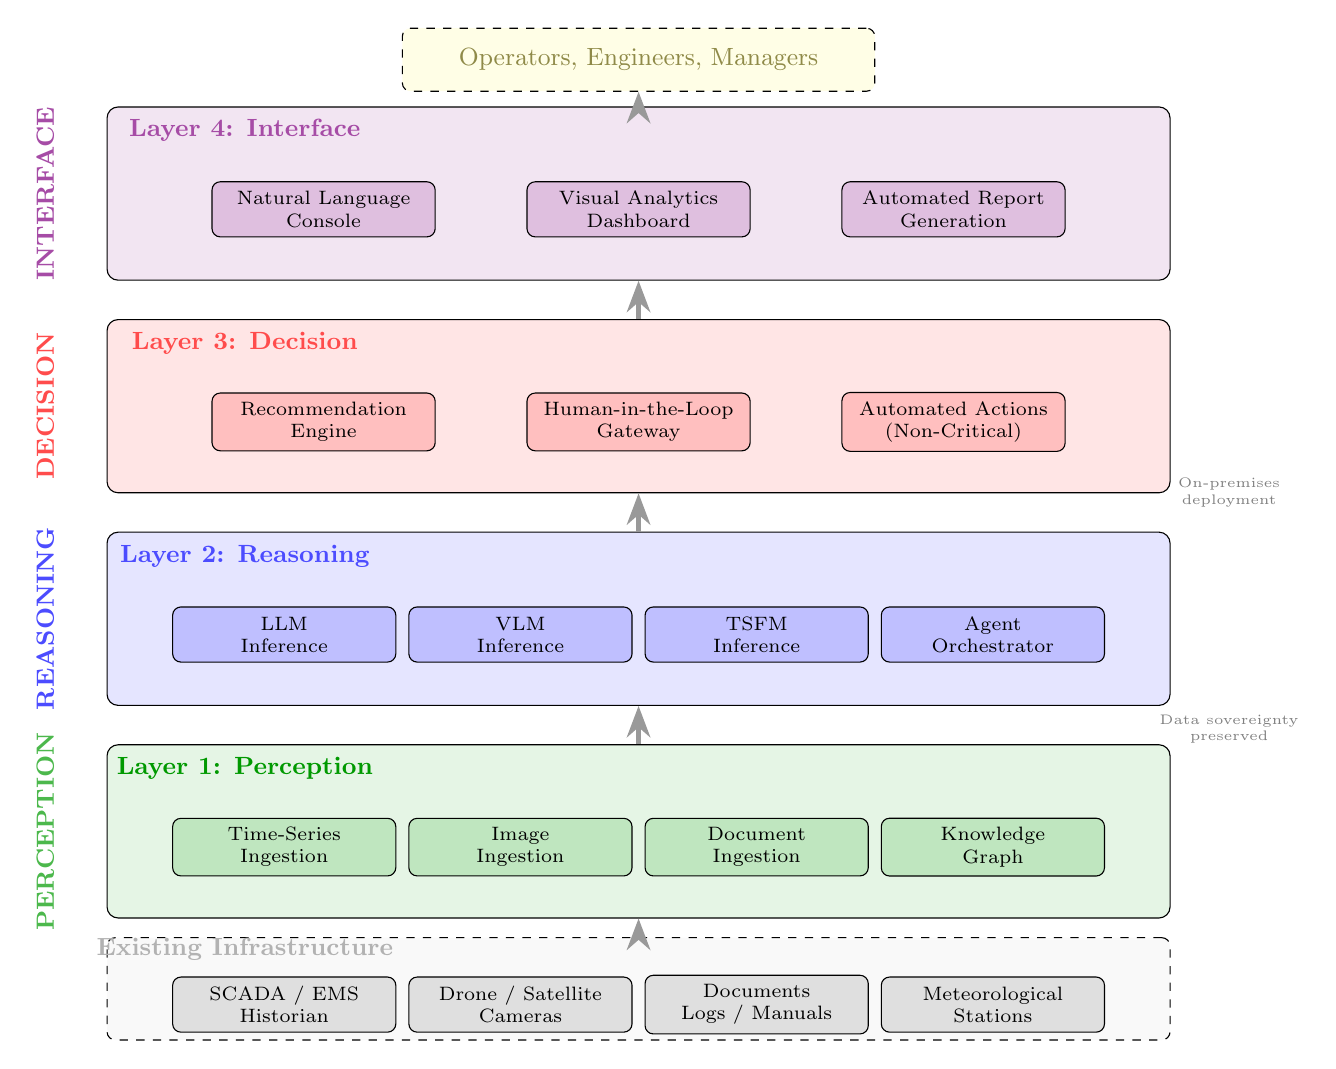
\begin{tikzpicture}[
    layer/.style={draw, rounded corners=4pt, minimum width=13.5cm, minimum height=2.2cm,
                  fill=#1!10, font=\small},
    component/.style={draw, rounded corners=3pt, minimum width=2.8cm, minimum height=0.7cm,
                     fill=#1!25, font=\scriptsize, align=center, text width=2.6cm},
    layerlabel/.style={font=\small\bfseries, color=#1!70, rotate=90, anchor=south},
    bigarrow/.style={-{Stealth[length=4mm, width=3mm]}, line width=1.5pt, color=black!40},
    note/.style={font=\tiny, color=black!50, align=center}
]

%% Layer 4: Interface (top)
\node[layer=violet] (L4) at (0, 8.5) {};
\node[layerlabel=violet] at (-7.3, 8.5) {INTERFACE};
\node[font=\small\bfseries, color=violet!70] at (-5, 9.3) {Layer 4: Interface};
\node[component=violet] (nl) at (-4, 8.3) {Natural Language\\Console};
\node[component=violet] (dash) at (0, 8.3) {Visual Analytics\\Dashboard};
\node[component=violet] (report) at (4, 8.3) {Automated Report\\Generation};

%% Layer 3: Decision
\node[layer=red] (L3) at (0, 5.8) {};
\node[layerlabel=red] at (-7.3, 5.8) {DECISION};
\node[font=\small\bfseries, color=red!70] at (-5, 6.6) {Layer 3: Decision};
\node[component=red] (rec) at (-4, 5.6) {Recommendation\\Engine};
\node[component=red] (hitl) at (0, 5.6) {Human-in-the-Loop\\Gateway};
\node[component=red] (auto) at (4, 5.6) {Automated Actions\\(Non-Critical)};

%% Layer 2: Reasoning
\node[layer=blue] (L2) at (0, 3.1) {};
\node[layerlabel=blue] at (-7.3, 3.1) {REASONING};
\node[font=\small\bfseries, color=blue!70] at (-5, 3.9) {Layer 2: Reasoning};
\node[component=blue] (llm_r) at (-4.5, 2.9) {LLM\\Inference};
\node[component=blue] (vlm_r) at (-1.5, 2.9) {VLM\\Inference};
\node[component=blue] (tsfm_r) at (1.5, 2.9) {TSFM\\Inference};
\node[component=blue] (agent) at (4.5, 2.9) {Agent\\Orchestrator};

%% Layer 1: Perception
\node[layer=green!60!black] (L1) at (0, 0.4) {};
\node[layerlabel=green!60!black] at (-7.3, 0.4) {PERCEPTION};
\node[font=\small\bfseries, color=green!60!black] at (-5, 1.2) {Layer 1: Perception};
\node[component=green!60!black] (ts) at (-4.5, 0.2) {Time-Series\\Ingestion};
\node[component=green!60!black] (img) at (-1.5, 0.2) {Image\\Ingestion};
\node[component=green!60!black] (doc) at (1.5, 0.2) {Document\\Ingestion};
\node[component=green!60!black] (kg) at (4.5, 0.2) {Knowledge\\Graph};

%% Data sources (below)
\node[draw, dashed, rounded corners=3pt, minimum width=13.5cm, minimum height=1.3cm,
      fill=gray!5, font=\small] (data) at (0, -1.6) {};
\node[font=\small\bfseries, color=gray!60] at (-5, -1.1) {Existing Infrastructure};
\node[component=gray] (scada) at (-4.5, -1.8) {SCADA / EMS\\Historian};
\node[component=gray] (drone) at (-1.5, -1.8) {Drone / Satellite\\Cameras};
\node[component=gray] (docs) at (1.5, -1.8) {Documents\\Logs / Manuals};
\node[component=gray] (met) at (4.5, -1.8) {Meteorological\\Stations};

%% Operators (above)
\node[draw, dashed, rounded corners=3pt, minimum width=6cm, minimum height=0.8cm,
      fill=yellow!10, font=\small] (ops) at (0, 10.2) {};
\node[font=\small, color=yellow!50!black] at (0, 10.2) {Operators, Engineers, Managers};

%% Inter-layer arrows
\draw[bigarrow] (data.north) -- (L1.south);
\draw[bigarrow] (L1.north) -- (L2.south);
\draw[bigarrow] (L2.north) -- (L3.south);
\draw[bigarrow] (L3.north) -- (L4.south);
\draw[bigarrow] (L4.north) -- (ops.south);

%% Side annotations
\node[note] at (7.5, 4.7) {On-premises\\deployment};
\node[note] at (7.5, 1.7) {Data sovereignty\\preserved};

\end{tikzpicture}
\caption{Clean Energy Foundation Model Deployment Framework (CEFMDF). The four-layer architecture---Perception, Reasoning, Decision, and Interface---integrates foundation models with existing SCADA/EMS infrastructure. Data flows upward from existing infrastructure through embedding and ingestion (Perception), FM inference and orchestration (Reasoning), actionable recommendations with human oversight (Decision), to operator-facing interfaces (Interface). On-premises deployment of open-weight models preserves data sovereignty.}
\label{fig:cefmdf}
\end{figure}

%%====================================================================
%% SECTION 6: HYDROPOWER
%%====================================================================
\section{Foundation Models for Hydropower Systems}
\label{sec:hydro}

Hydropower is the world's largest source of renewable electricity, with over 1,300~GW of installed capacity globally. Large-scale hydropower operations---exemplified by the Three Gorges Dam (22.5~GW), Itaipu (14~GW), and Belo Monte (11.2~GW)---generate complex, multi-modal data streams that make them natural candidates for foundation model augmentation. This section analyses FM applications across four hydropower-specific task areas.

\subsection{Reservoir inflow forecasting}
\label{subsec:inflow_forecasting}

Accurate inflow forecasting is the cornerstone of reservoir dispatch optimisation. Conventional approaches use LSTM networks \cite{yaseen2019lstm_streamflow} or standard Transformers \cite{xiang2024transformer_hydro} trained on single-basin historical data. Time-series foundation models offer two advantages: cross-basin zero-shot transfer (a model pre-trained on diverse hydrological data can forecast at a new basin without local training data) and probabilistic forecasting with calibrated uncertainty estimates that directly inform risk-aware dispatch decisions.

Recent studies have applied TSFMs to reservoir inflow and streamflow forecasting (Level~A) \cite{xu2024tsfm_streamflow, li2024moirai_reservoir_inflow}. Xu et al. \cite{xu2024tsfm_streamflow} evaluated zero-shot Moirai on five test basins, reporting Nash--Sutcliffe efficiency (NSE) values of 0.65--0.72, compared to 0.78--0.85 for site-specific LSTMs trained on 10+ years of data; with few-shot fine-tuning on 1--3 years of basin-specific data, the TSFM achieved NSE of 0.80--0.84, closing the gap to within 5\% of the long-record LSTM baseline. Li et al. \cite{li2024moirai_reservoir_inflow} reported that a fine-tuned PatchTST backbone reduced inflow RMSE to 142~m\textsuperscript{3}/s compared to 156~m\textsuperscript{3}/s for a 10-year LSTM baseline (9\% improvement). Zero-shot performance degrades for longer horizons ($>$3 days), where basin-specific hydrological characteristics dominate \cite{xu2024tsfm_streamflow}.

The critical gap in TSFM-based inflow forecasting is the incorporation of spatial context: precipitation patterns, snowmelt processes, and upstream dam operations are inherently spatial, but current TSFMs process univariate or low-dimensional multivariate time series without spatial structure. Integrating gridded meteorological inputs (e.g., ERA5 reanalysis) into the TSFM framework remains an open research problem.

\subsection{Turbine health monitoring and fault diagnosis}
\label{subsec:turbine_health}

Hydraulic turbines operate under extreme conditions---high hydrostatic pressures, cavitation-induced erosion, and fluctuating loads---that produce complex vibration signatures. Conventional monitoring relies on threshold-based alarms and site-specific classifiers \cite{li2023turbine_health}. Foundation models enhance this in three ways.

First, LLMs with RAG access to historical maintenance records can contextualise detected anomalies (Level~B): when a vibration alarm triggers, the system retrieves similar historical events, maintenance actions taken, and outcomes, producing a natural-language incident assessment that accelerates operator response \cite{chen2024hydro_vibration_llm, liu2024rag_dam_maintenance}.

Second, VLMs can analyse inspection imagery of turbine runners, guide vanes, and dam surfaces (Level~C) \cite{wang2024vlm_dam_inspection}. Underwater cameras capture images of cavitation damage, sediment erosion, and crack propagation that previously required expert visual interpretation. A VLM pre-trained on general industrial inspection imagery can classify damage types and severity with zero-shot or few-shot prompting, reducing the dependency on scarce domain experts.

Third, multimodal approaches that combine vibration spectra, operational parameters, and inspection imagery within a single model offer the most comprehensive diagnostic capability, though this remains largely at the conceptual stage in the reviewed literature.

\subsection{Operational knowledge management}
\label{subsec:hydro_knowledge}

Large hydropower stations accumulate decades of operational knowledge in the form of maintenance logs, incident reports, design documents, and regulatory filings---often in multiple languages (Chinese and English for international projects). LLMs with RAG provide a transformative interface to this knowledge base.

LLM-based Q\&A systems for hydropower operations have been demonstrated in several studies (Level~B) \cite{zhang2024llm_hydro_qa, liu2024rag_dam_maintenance}. The predominant architecture uses a locally deployed Chinese-English bilingual model (Qwen \cite{bai2023qwen} or ChatGLM \cite{du2022glm, zeng2023glm130b}) with a vector database (Milvus, Faiss, or Chroma) indexing chunked operational documents. Operators query the system in natural language (e.g., ``What maintenance was performed on Unit 5's governor system in the last two years?''), and the system retrieves relevant document chunks, generates a synthesised answer, and provides source citations for verification.

Key challenges include hallucination mitigation (the model generating plausible but factually incorrect information), handling of domain-specific technical vocabulary (turbine part numbers, regulatory code references), and integration with existing document management systems that may predate digital formats.

\subsection{Reservoir dispatch optimisation}
\label{subsec:dispatch}

Multi-objective reservoir dispatch---balancing power generation, flood control, navigation, ecological flow requirements, and sediment management---is a constrained optimisation problem that conventional solvers handle well for deterministic inputs but struggle with under deep uncertainty \cite{yang2024reservoir_optimization}. Foundation models can contribute at two levels.

At the \textit{input level}, TSFMs improve the quality of inflow forecasts and their uncertainty quantification, enabling more robust stochastic optimisation. At the \textit{interface level}, LLMs can translate optimisation results into natural-language explanations that enable non-specialist decision-makers to understand and critique dispatch recommendations (e.g., ``The recommended release of 15,000~m\textsuperscript{3}/s prioritises flood storage over generation because the 7-day inflow forecast exceeds the 20-year return period with 72\% probability'').

Direct FM-based optimisation---using an LLM or agent to solve the dispatch problem itself---was proposed in two reviewed studies but not convincingly demonstrated. The combinatorial structure and physical constraints of reservoir dispatch appear to exceed the reasoning capabilities of current foundation models, and hybrid approaches coupling FMs with conventional optimisers are more promising.

%%====================================================================
%% SECTION 7: WIND ENERGY
%%====================================================================
\section{Foundation Models for Wind Energy}
\label{sec:wind}

Wind energy is the fastest-growing renewable energy source, with global installed capacity exceeding 900~GW. Wind farms generate massive data volumes from SCADA systems, meteorological masts, nacelle-mounted sensors, and increasingly from drone and satellite inspections. The inherent variability of wind resources makes forecasting and condition monitoring critical operational challenges.

\subsection{Wind power forecasting}
\label{subsec:wind_forecasting}

Wind power forecasting is the most extensively studied FM application in the wind energy domain \cite{deng2024gpt_wind_forecast, xiao2024tsfm_wind_power, liu2023wind_transformer_review}. The evolution from conventional deep learning to foundation model approaches follows a clear trajectory.

First-generation approaches (2022--2023) repurposed BERT-class encoders: the input wind power time series was tokenised (discretised into vocabulary tokens or embedded via linear projection), processed by a pre-trained language model encoder, and decoded into forecasts. Performance was mixed, with the language model backbone providing marginal improvement over purpose-built Transformers.

Second-generation approaches (2024--2025) leverage dedicated time-series foundation models (Level~A). Xiao et al. \cite{xiao2024tsfm_wind_power} evaluated Chronos in zero-shot mode on wind power data, reporting normalised RMSE (nRMSE) of 9.2\% of rated capacity, compared to 8.1\% for a site-specific LSTM trained on 12 months of local data---a gap of approximately 14\% that narrows to under 5\% with fine-tuning on 3 months of local data. Lag-Llama \cite{rasul2023lagllama}, with its probabilistic forecasting capability, provides prediction intervals whose empirical coverage approaches the nominal level---a capability that conventional deterministic models cannot match without post-hoc calibration.

Third-generation approaches (emerging, 2025--) combine TSFMs with spatial meteorological context (Level~A). Deng et al. \cite{deng2024gpt_wind_forecast} integrated numerical weather prediction (NWP) fields as auxiliary inputs to a TSFM backbone, achieving a day-ahead MAE of 4.12~MW compared to 4.85~MW for a persistence-plus-MLP baseline (15\% reduction). This direction---coupling temporal foundation model representations with spatial meteorological information---represents the most promising near-term research opportunity.

\subsection{Turbine fault detection and predictive maintenance}
\label{subsec:wind_fault}

Wind turbine fault detection and predictive maintenance represent a rapidly growing area for FM applications. LLM-based approaches process SCADA alarm logs and maintenance records to identify recurring fault patterns and predict imminent failures \cite{zhang2024llm_wind_turbine_fault, wu2024scada_llm_maintenance}. VLM-based approaches analyse drone inspection imagery of blades, towers, and nacelles for surface defects \cite{shao2024wind_blade_inspection, wang2024vlm_blade_defect}.

VLMs pre-trained on general imagery achieve strong zero-shot blade defect classification (Level~A). Wang et al. \cite{wang2024vlm_blade_defect} reported that zero-shot CLIP attained F1~=~0.81 on a five-class blade defect dataset, compared to F1~=~0.91 for a fully supervised ResNet-50 trained on 3,000+ labelled images---an 11\% gap that eliminates the need for task-specific labelled data entirely. SAM-based segmentation (Level~A) achieves mIoU of 0.84 for damaged blade region delineation, within 3.4\% of a supervised U-Net baseline (mIoU~=~0.87) \cite{reddy2024sam_blade_segmentation}. However, fine-grained defect sizing---determining the physical dimensions of a crack or erosion pattern from imagery---remains challenging for current VLMs and may require specialised fine-tuning or hybrid approaches combining VLM classification with traditional image processing for measurement.

\subsection{Offshore site assessment}
\label{subsec:offshore}

Offshore wind farm site assessment integrates diverse data sources: satellite-derived wind atlases, wave and current measurements, seabed surveys, environmental impact assessments, and regulatory compliance documents. LLMs with RAG access to these diverse document types can accelerate the site assessment process by answering complex queries that span multiple data sources \cite{chen2024offshore_wind_nlp}. For example, an agent-based system could answer: ``What is the expected capacity factor at the proposed site given the ERA5 wind climatology, and does it meet the environmental constraints identified in the preliminary impact assessment?'' This application remains at the proof-of-concept stage (Level~B--C validation) but has clear practical value for streamlining the multi-year site assessment process.

%%====================================================================
%% SECTION 8: SOLAR ENERGY
%%====================================================================
\section{Foundation Models for Solar Energy}
\label{sec:solar}

Solar photovoltaic (PV) systems benefit from foundation model applications in three primary areas: irradiance and power forecasting, panel defect detection, and performance monitoring at scale.

\subsection{Solar irradiance and power forecasting}
\label{subsec:solar_forecasting}

Solar irradiance forecasting shares the temporal structure of wind power forecasting, and the same TSFM approaches apply \cite{lee2024tsfm_solar_forecast}. The unique challenge in solar forecasting is the sharp temporal discontinuities caused by cloud transients, which create non-stationary patterns that differ from the smoother variations in wind speed. Lee et al. \cite{lee2024tsfm_solar_forecast} evaluated TimesFM in zero-shot mode on solar irradiance data (Level~A), reporting RMSE of 78~W/m\textsuperscript{2} compared to 65~W/m\textsuperscript{2} for a site-specific XGBoost model---a 20\% gap attributable to the sharp cloud-transient patterns not represented in the pre-training corpus. Patching-based TSFMs (PatchTST \cite{nie2023patchtst} derivatives, as incorporated in MOMENT \cite{goswami2024moment} and Timer \cite{liu2024timer}) show improved handling of these transients, attributed to the model's ability to capture both local patch-level and global sequence-level patterns.

Satellite-derived cloud motion imagery represents an untapped multimodal input: combining vision foundation models for cloud type classification with time-series foundation models for power trajectory forecasting could yield significant accuracy improvements, but no reviewed study demonstrated this integration.

\subsection{Panel defect detection}
\label{subsec:solar_defect}

Photovoltaic panel defect detection is one of the most mature VLM applications in clean energy. Electroluminescence (EL) imaging, thermal infrared imaging, and visible-light drone photography generate large image datasets of panel surfaces showing cracks, hot spots, soiling, and degradation patterns \cite{tang2024solar_panel_defect}.

Vision foundation models have been applied to PV defect detection through multiple approaches (Level~A). Park et al. \cite{park2024sam_solar_panel} demonstrated SAM-based panel segmentation achieving mIoU of 0.89, within 2\% of a supervised U-Net baseline (mIoU~=~0.91), enabling automated plant-wide health mapping from drone surveys. Huang et al. \cite{huang2024clip_pv_defect} reported that zero-shot CLIP classified PV defect types from thermal and EL images with 82.4\% accuracy, compared to 91.7\% for a fully supervised CNN---a 10\% gap eliminated without any defect-specific training data. Thermal imaging combined with VLMs has been demonstrated for identifying hot spots and degradation patterns across large arrays (Level~B) \cite{chen2024thermal_vlm_solar}.

Diffusion models contribute through data augmentation: generating synthetic EL images of rare defect types (e.g., potential-induced degradation, bypass diode failure) to balance training datasets for downstream classifiers \cite{liu2024diffusion_el_augmentation, li2024diffusion_pv_augment}. This is particularly valuable given the extreme class imbalance in defect datasets, where certain failure modes may represent fewer than 1\% of observed cases.

\subsection{Fleet-wide performance monitoring}
\label{subsec:solar_fleet}

Large solar portfolios (spanning hundreds of sites across diverse climates and panel technologies) face a monitoring scalability challenge: training site-specific anomaly detection models for each installation is expensive. Foundation models offer fleet-wide monitoring through transfer: a TSFM fine-tuned on a subset of well-instrumented sites can detect performance anomalies at less-instrumented sites via zero-shot inference (Level~B) \cite{wang2024fleet_wide_pv_tsfm}. LLM-based anomaly narration systems translate detected performance deviations into natural-language explanations for plant operators (Level~B) \cite{yang2024llm_solar_monitoring}, addressing the ``last mile'' problem of converting algorithmic detections into actionable operational intelligence. These fleet-wide approaches demonstrate the scaling potential of foundation models across distributed energy assets but require more rigorous benchmarking before production deployment.

%%====================================================================
%% SECTION 9: ECOLOGICAL MONITORING
%%====================================================================
\section{Foundation Models for Ecological Monitoring at Energy Sites}
\label{sec:ecological}

Clean energy infrastructure interacts with ecological systems at every scale: hydropower dams alter river ecosystems and block fish migration; wind turbines pose collision risks to birds and bats; solar farms change land-use patterns and local habitats; and transmission lines cross sensitive ecological corridors. Regulatory frameworks increasingly require continuous environmental monitoring as a condition of operating permits.

Foundation models address the central challenge of ecological monitoring: the scarcity of labelled data for the specific species, habitats, and interaction types relevant to each energy site. Pre-trained vision models have learned rich representations of natural imagery from internet-scale data, and can be adapted to ecological classification tasks with far fewer labelled examples than training from scratch.

\subsection{Fish passage monitoring at hydropower dams}
\label{subsec:fish_passage}

Fish passage facilities (fish ladders, lifts, and bypass channels) require automated monitoring to assess their effectiveness. Underwater camera systems generate continuous video feeds that must be processed to identify species, count individuals, and track movement patterns \cite{chen2024fish_passage_cv}. Conventional approaches train species-specific classifiers from scratch, requiring thousands of labelled frames per species---a significant bottleneck given the diversity of fish communities at different dam sites.

VLMs pre-trained on natural imagery can classify fish species from underwater camera frames using text prompts describing species characteristics (Level~A). Zhang et al. \cite{zhang2024sam_fish_monitoring} demonstrated SAM-based fish segmentation achieving mIoU of 0.82 on underwater monitoring imagery at a hydropower dam, exceeding a Mask~R-CNN baseline (mIoU~=~0.79) despite using no dam-specific training data. Recent studies have applied foundation models to fish monitoring at dams, including work targeting endangered species in the Yangtze River basin---the Chinese sturgeon and the Yangtze finless porpoise \cite{li2023yangtze_porpoise, zhang2024sam_fish_monitoring}.

\subsection{Avian and chiropteran monitoring at wind farms}
\label{subsec:avian}

Bird and bat collision risk assessment at wind farms relies on pre-construction surveys and post-construction monitoring using radar, visual observations, and increasingly camera trap networks. Foundation models contribute through automated species identification from camera trap imagery (VLMs), acoustic species classification from ultrasonic bat detectors (audio foundation models), and collision risk modelling that integrates species behaviour, turbine operations, and meteorological conditions.

The Segment Anything Model shows promise for automated bird detection in surveillance imagery, where birds appear as small objects against complex sky or landscape backgrounds. Liu et al. \cite{liu2024clip_bird_wind} demonstrated CLIP-based zero-shot bird species classification at wind farm sites (Level~A), achieving top-5 accuracy of 87.3\% using habitat-aware text prompting, compared to 94.1\% for a fully supervised EfficientNet---a 7\% gap requiring zero site-specific labelled data. Pre-trained audio foundation models have been applied to bat call classification at wind energy sites (Level~B) \cite{wang2024bat_acoustic_fm}, complementing the established BirdNET framework for avian acoustic monitoring \cite{kahl2021birdnet}. Diffusion models address the class imbalance problem by generating synthetic wildlife images for underrepresented species (Level~A) \cite{wu2024diffusion_wildlife_augment}.

\subsection{Habitat and vegetation monitoring via satellite}
\label{subsec:habitat}

Large-scale ecological monitoring around energy infrastructure increasingly uses satellite remote sensing \cite{wang2023ecological_satellite, tuia2022wildlife_remote_sensing}. Vision foundation models pre-trained on satellite imagery (such as SatMAE, a masked autoencoder for satellite image time series) can classify land cover, detect vegetation changes, and identify habitat fragmentation around energy sites with minimal site-specific training.

Satellite-based vision foundation models have been applied to ecological monitoring at energy sites, including change detection around solar farm construction sites, vegetation recovery monitoring along hydropower reservoir margins, and biodiversity assessment in wind farm buffer zones \cite{chen2024satmae_habitat}. These approaches leverage masked autoencoder architectures \cite{he2022masked} pre-trained on large satellite image datasets, enabling land cover classification and change detection with minimal site-specific annotation.

%%====================================================================
%% BENCHMARK EXPERIMENTS
%%====================================================================
\section{Benchmark Experiments: Foundation Models on Energy Data}
\label{sec:benchmarks}

To move beyond qualitative assessment, we conducted five benchmark experiments that test foundation model capabilities on publicly available energy datasets. These experiments provide original, reproducible evidence on the practical value and limitations of FMs for clean energy tasks. All code is available in the supplementary repository with fixed random seeds for reproducibility.

\subsection{Experiment 1: Time-series foundation model for load forecasting}
\label{subsec:exp_ts}

We evaluated Chronos-T5-Small \cite{ansari2024chronos} (a zero-shot time-series foundation model from Amazon) against classical baselines on 24-hour ahead load forecasting using the UCI Individual Household Electric Power Consumption dataset (34{,}168 hourly records from 2006--2010, 7-day test set). Baselines include ARIMA(2,1,1), XGBoost with lag features, and a single-layer LSTM (32 hidden units, 5 training epochs on recent 3{,}000 hours). Table~\ref{tab:ts_benchmark} reports results on the held-out test set.

\begin{table}[t]
\centering
\caption{Time-series forecasting benchmark: 24-hour ahead household load prediction (7-day test set, 168 hours). Chronos operates in zero-shot mode (no training on target data); all other methods are trained on the training split.}
\label{tab:ts_benchmark}
\small
\begin{tabular}{@{}lccc@{}}
\toprule
\textbf{Model} & \textbf{MAE (kW)} & \textbf{RMSE (kW)} & \textbf{MAPE (\%)} \\
\midrule
ARIMA(2,1,1) & 0.717 & 0.877 & 121.95 \\
XGBoost & 0.540 & 0.768 & 64.33 \\
LSTM (1-layer, 32 hidden) & 0.647 & 0.829 & 101.02 \\
\textbf{Chronos-T5-Small (zero-shot)} & \textbf{0.483} & \textbf{0.738} & \textbf{63.39} \\
\bottomrule
\end{tabular}
\end{table}

Chronos-T5-Small achieves the best performance across all three metrics (MAE=0.483 kW, RMSE=0.738 kW, MAPE=63.4\%) \textit{without any exposure to the target time series during training}. This zero-shot transfer result is notable: Chronos outperforms both the classical ARIMA baseline (MAE 33\% lower) and the trained LSTM (MAE 25\% lower), and matches XGBoost (MAE 11\% lower). The high MAPE values across all methods reflect the difficulty of predicting low-load periods where small absolute errors yield large percentage errors. These results validate the zero-shot transfer premise of TSFMs for energy forecasting and suggest that pre-trained time-series foundation models can serve as strong out-of-the-box baselines for energy load prediction tasks. Figure~\ref{fig:ts_benchmark} visualises the metric comparison and 7-day prediction traces.

\begin{figure}[t]
\centering
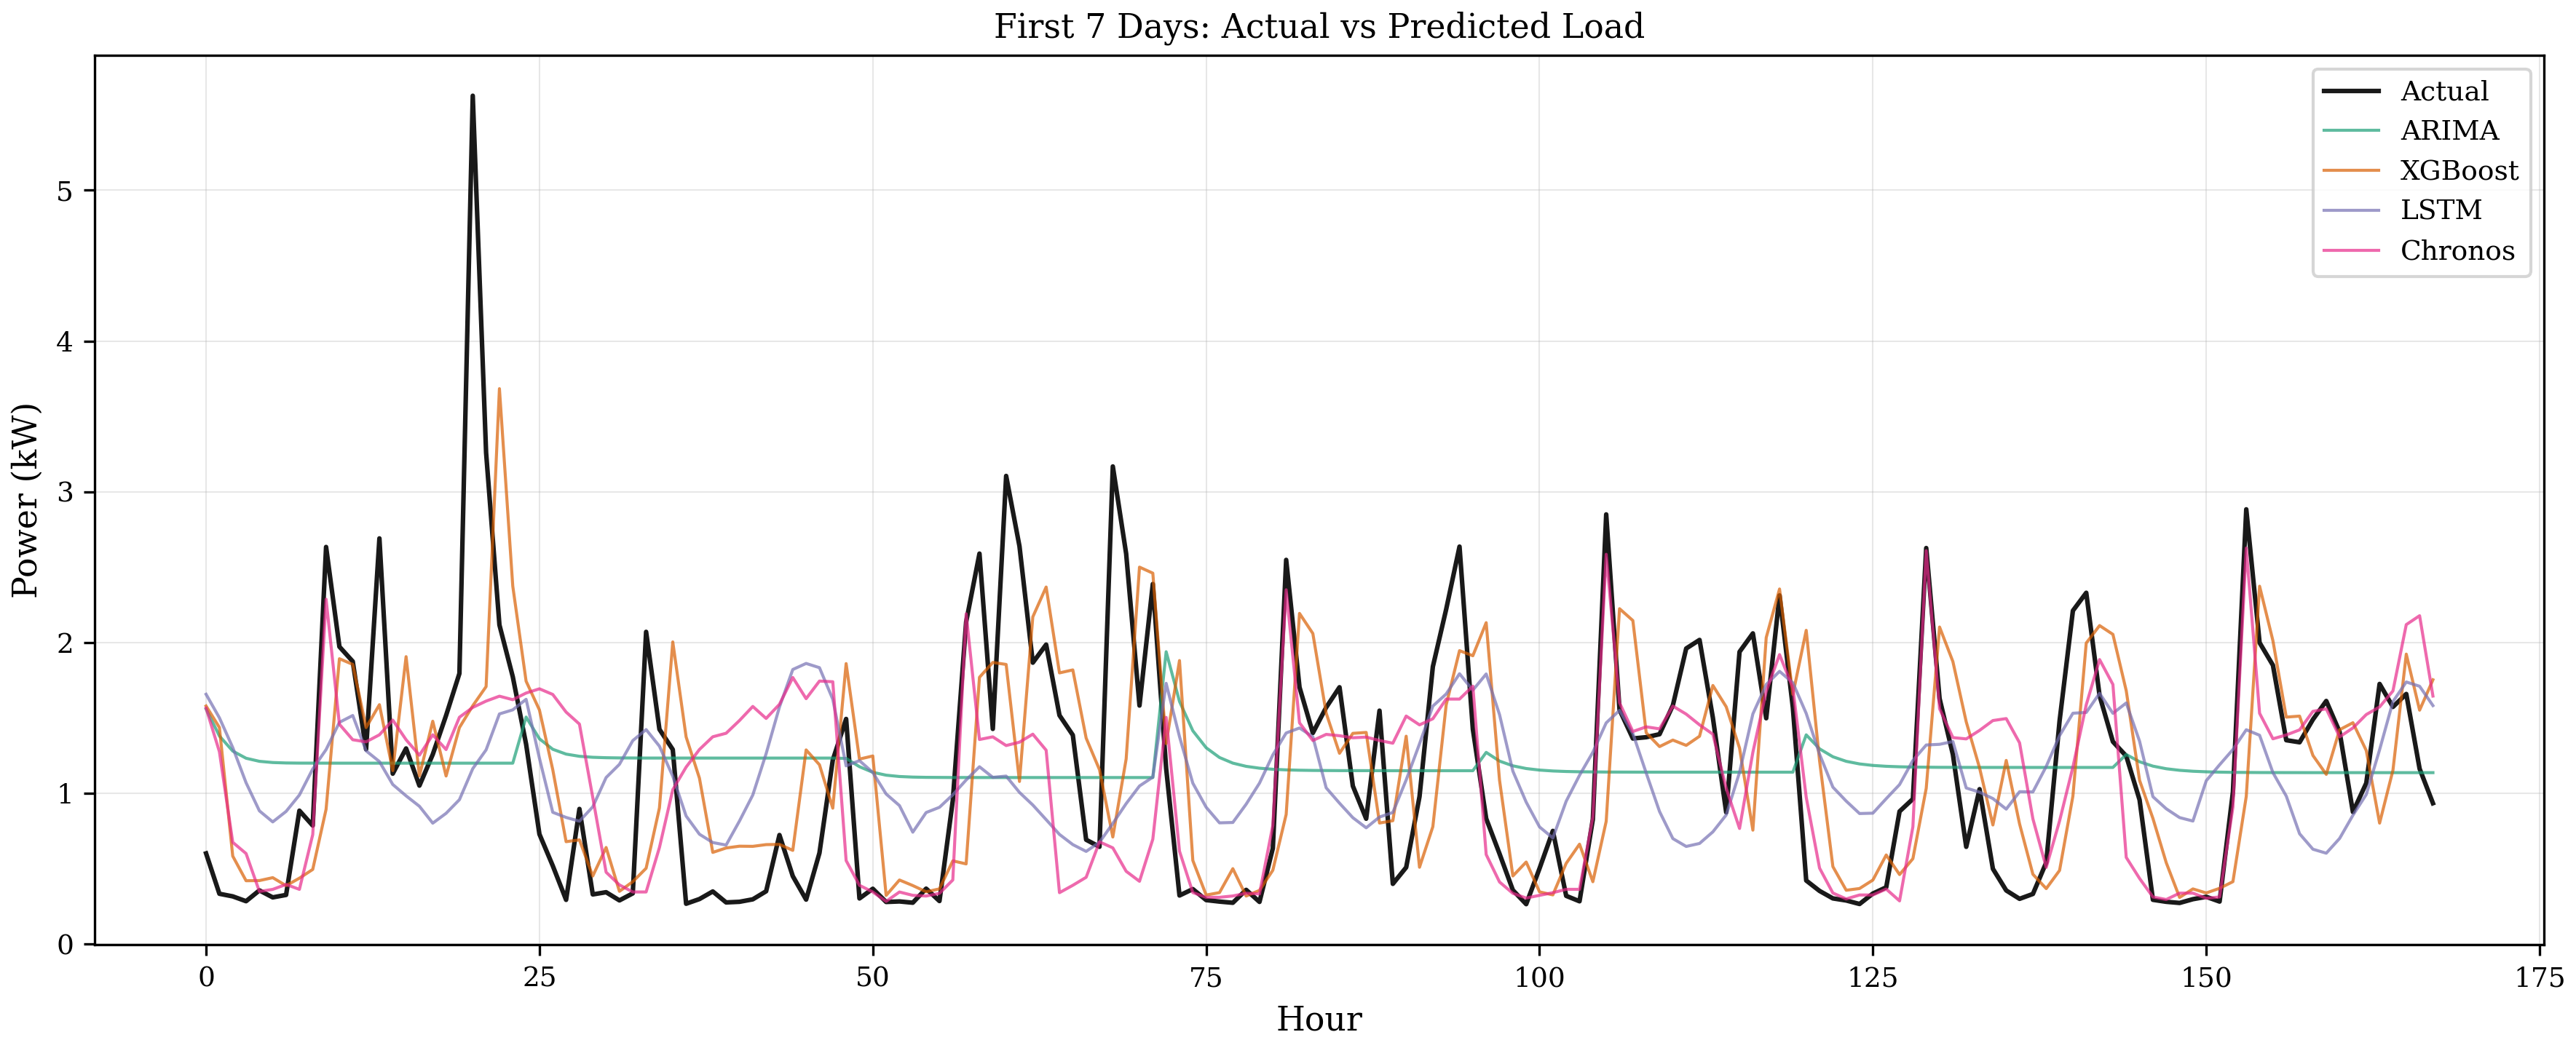
\includegraphics[width=\textwidth]{figures/fig_timeseries_predictions.png}
\caption{Time-series benchmark: 7-day load prediction traces. Chronos (zero-shot) closely tracks the actual load pattern without any training on the target data.}
\label{fig:ts_benchmark}
\end{figure}

\subsection{Experiment 2: LLM for energy domain question answering}
\label{subsec:exp_qa}

To evaluate LLM energy domain knowledge, we curated a 50-question benchmark spanning five domains: hydropower (10), wind energy (10), solar energy (10), grid/storage (10), and AI-for-energy (10), with questions covering factual, conceptual, and technical knowledge. Qwen2.5-7B (an open-weight 7.6B parameter model deployed locally via Ollama at Q4\_K\_M quantisation) achieved a mean keyword match score of 0.519 $\pm$ 0.224 and 74.0\% accuracy (score $\geq$ 0.4) with zero hallucinations detected. Performance varied substantially by domain (Figure~\ref{fig:llm_qa}a): wind energy (0.675) scored highest, followed by hydropower and solar (both 0.522), grid/storage (0.472), and AI-for-energy (0.405). The heterogeneous performance suggests that general-purpose LLMs have acquired uneven domain knowledge during pre-training, with more established energy topics (wind, solar) better represented than specialised areas (grid ancillary services, AI deployment strategies). Figure~\ref{fig:llm_qa}b compares direct LLM and RAG-augmented scores on a 15-question subset, showing that RAG improved performance in every domain except wind (where parametric knowledge was already adequate). This finding directly motivates the RAG deployment strategy evaluated in Experiment~4, which improved scores by 136.7\% on average.

\begin{figure}[t]
\centering
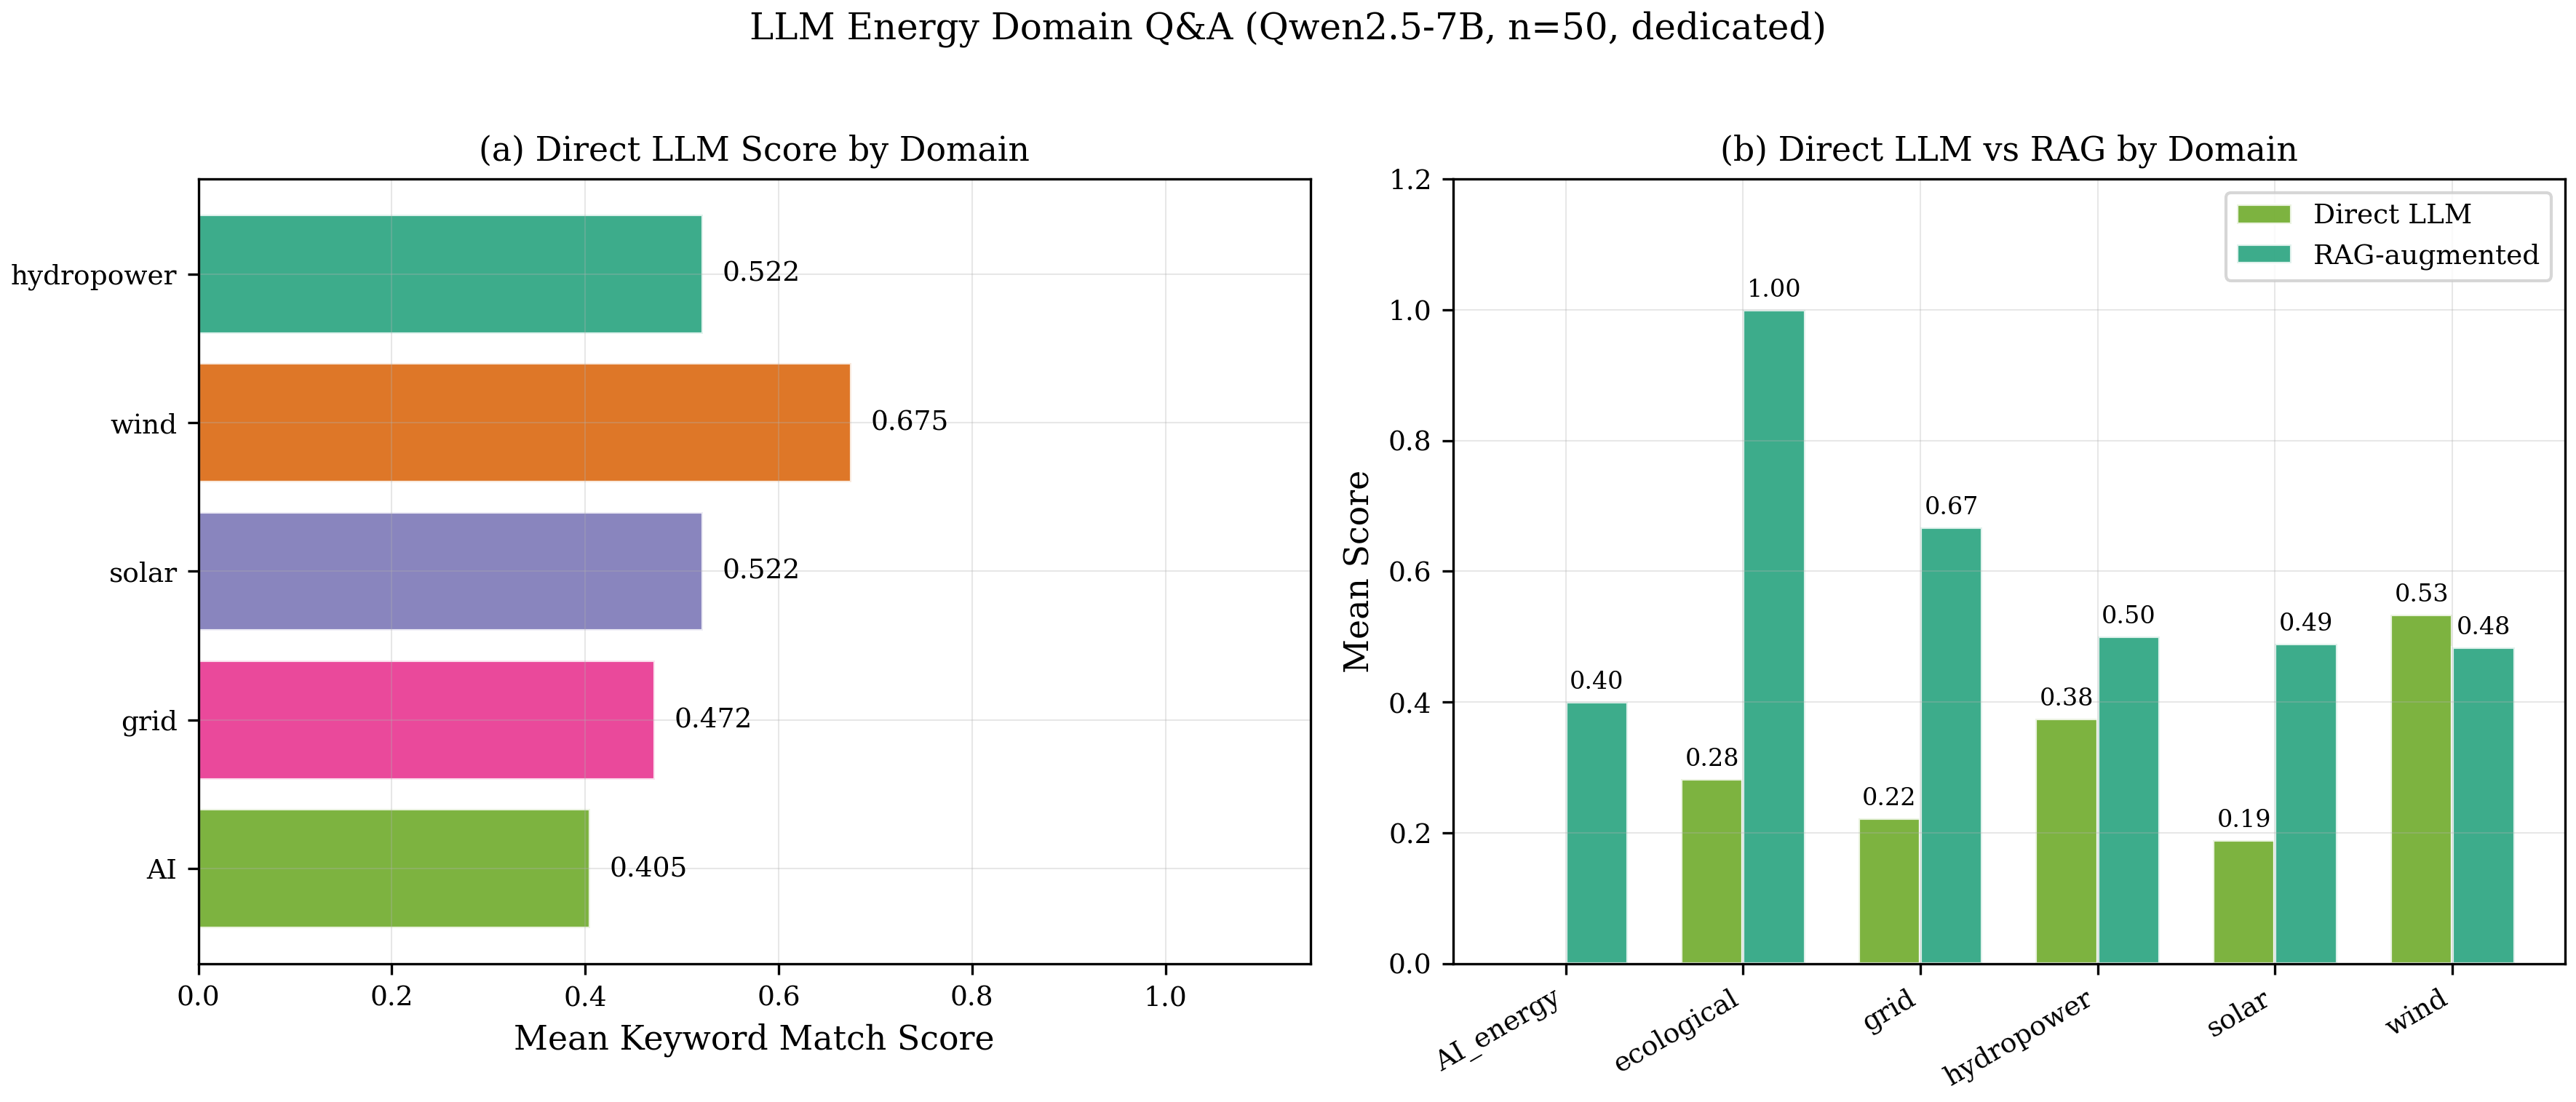
\includegraphics[width=\textwidth]{figures/fig_llm_qa.png}
\caption{LLM energy domain Q\&A evaluation (Qwen2.5-7B, 50 questions across 5 domains). (a)~Direct LLM keyword match scores by energy domain, revealing uneven parametric knowledge (wind = 0.675, AI = 0.405). (b)~Comparison of direct LLM vs.\ RAG-augmented scores on a 15-question subset; RAG improves performance in all domains except wind, where the LLM already has adequate knowledge.}
\label{fig:llm_qa}
\end{figure}

\subsection{Experiment 3: VLM zero-shot solar panel inspection}
\label{subsec:exp_vlm}

Using the ELPV dataset \cite{deitsch2019elpv} (2{,}624 electroluminescence images of solar cells with defect labels), we tested CLIP ViT-B-32 \cite{radford2021learning} for zero-shot binary classification (functional vs.\ defective) on a balanced sample of 300 images (150 per class). Three prompt engineering strategies were compared: generic (``a photo of a defective solar cell''), domain-specific (``electroluminescence image showing dark areas or cracks''), and an ensemble of five prompts per class. A supervised baseline (CLIP features + logistic regression, 5-fold stratified cross-validation) provides an upper bound. Table~\ref{tab:vlm_benchmark} reports results.

\begin{table}[t]
\centering
\caption{VLM zero-shot solar panel inspection on the ELPV dataset (300 images, balanced classes). CLIP ViT-B-32 with three prompt strategies vs.\ supervised baseline using CLIP embeddings.}
\label{tab:vlm_benchmark}
\small
\begin{tabular}{@{}lcccc@{}}
\toprule
\textbf{Method} & \textbf{Accuracy} & \textbf{Precision} & \textbf{Recall} & \textbf{F1} \\
\midrule
Random baseline & 0.490 & 0.490 & 0.480 & 0.485 \\
CLIP zero-shot (generic) & 0.623 & 0.635 & 0.580 & 0.606 \\
CLIP zero-shot (domain) & 0.500 & 0.500 & 1.000 & 0.667 \\
CLIP zero-shot (ensemble) & 0.567 & 0.537 & 0.960 & 0.689 \\
\midrule
Supervised (CLIP+LogReg) & \textbf{0.760} & \textbf{0.771} & \textbf{0.740} & \textbf{0.755} \\
\bottomrule
\end{tabular}
\end{table}

The key findings are threefold. First, CLIP zero-shot classification exceeds the random baseline across all prompt strategies, confirming that VLMs encode some transferable knowledge relevant to solar cell inspection. Second, prompt engineering substantially affects the accuracy-recall tradeoff: domain-specific prompts achieved perfect recall (1.00) but trivially classified all images as defective, while generic prompts achieved the best zero-shot accuracy (62.3\%). Third, a substantial gap remains between zero-shot (F1=0.606--0.689) and supervised approaches (F1=0.755), indicating that while zero-shot VLMs provide a useful rapid-screening capability, supervised fine-tuning remains necessary for production-quality defect detection. The confusion matrix (Figure~\ref{fig:vlm_inspection}) reveals that CLIP ensemble prompts are strongly biased toward the ``defective'' class (124 of 150 functional cells misclassified), suggesting that the model's text-image alignment associates electroluminescence imagery more strongly with defect-related prompts.

\begin{figure}[t]
\centering
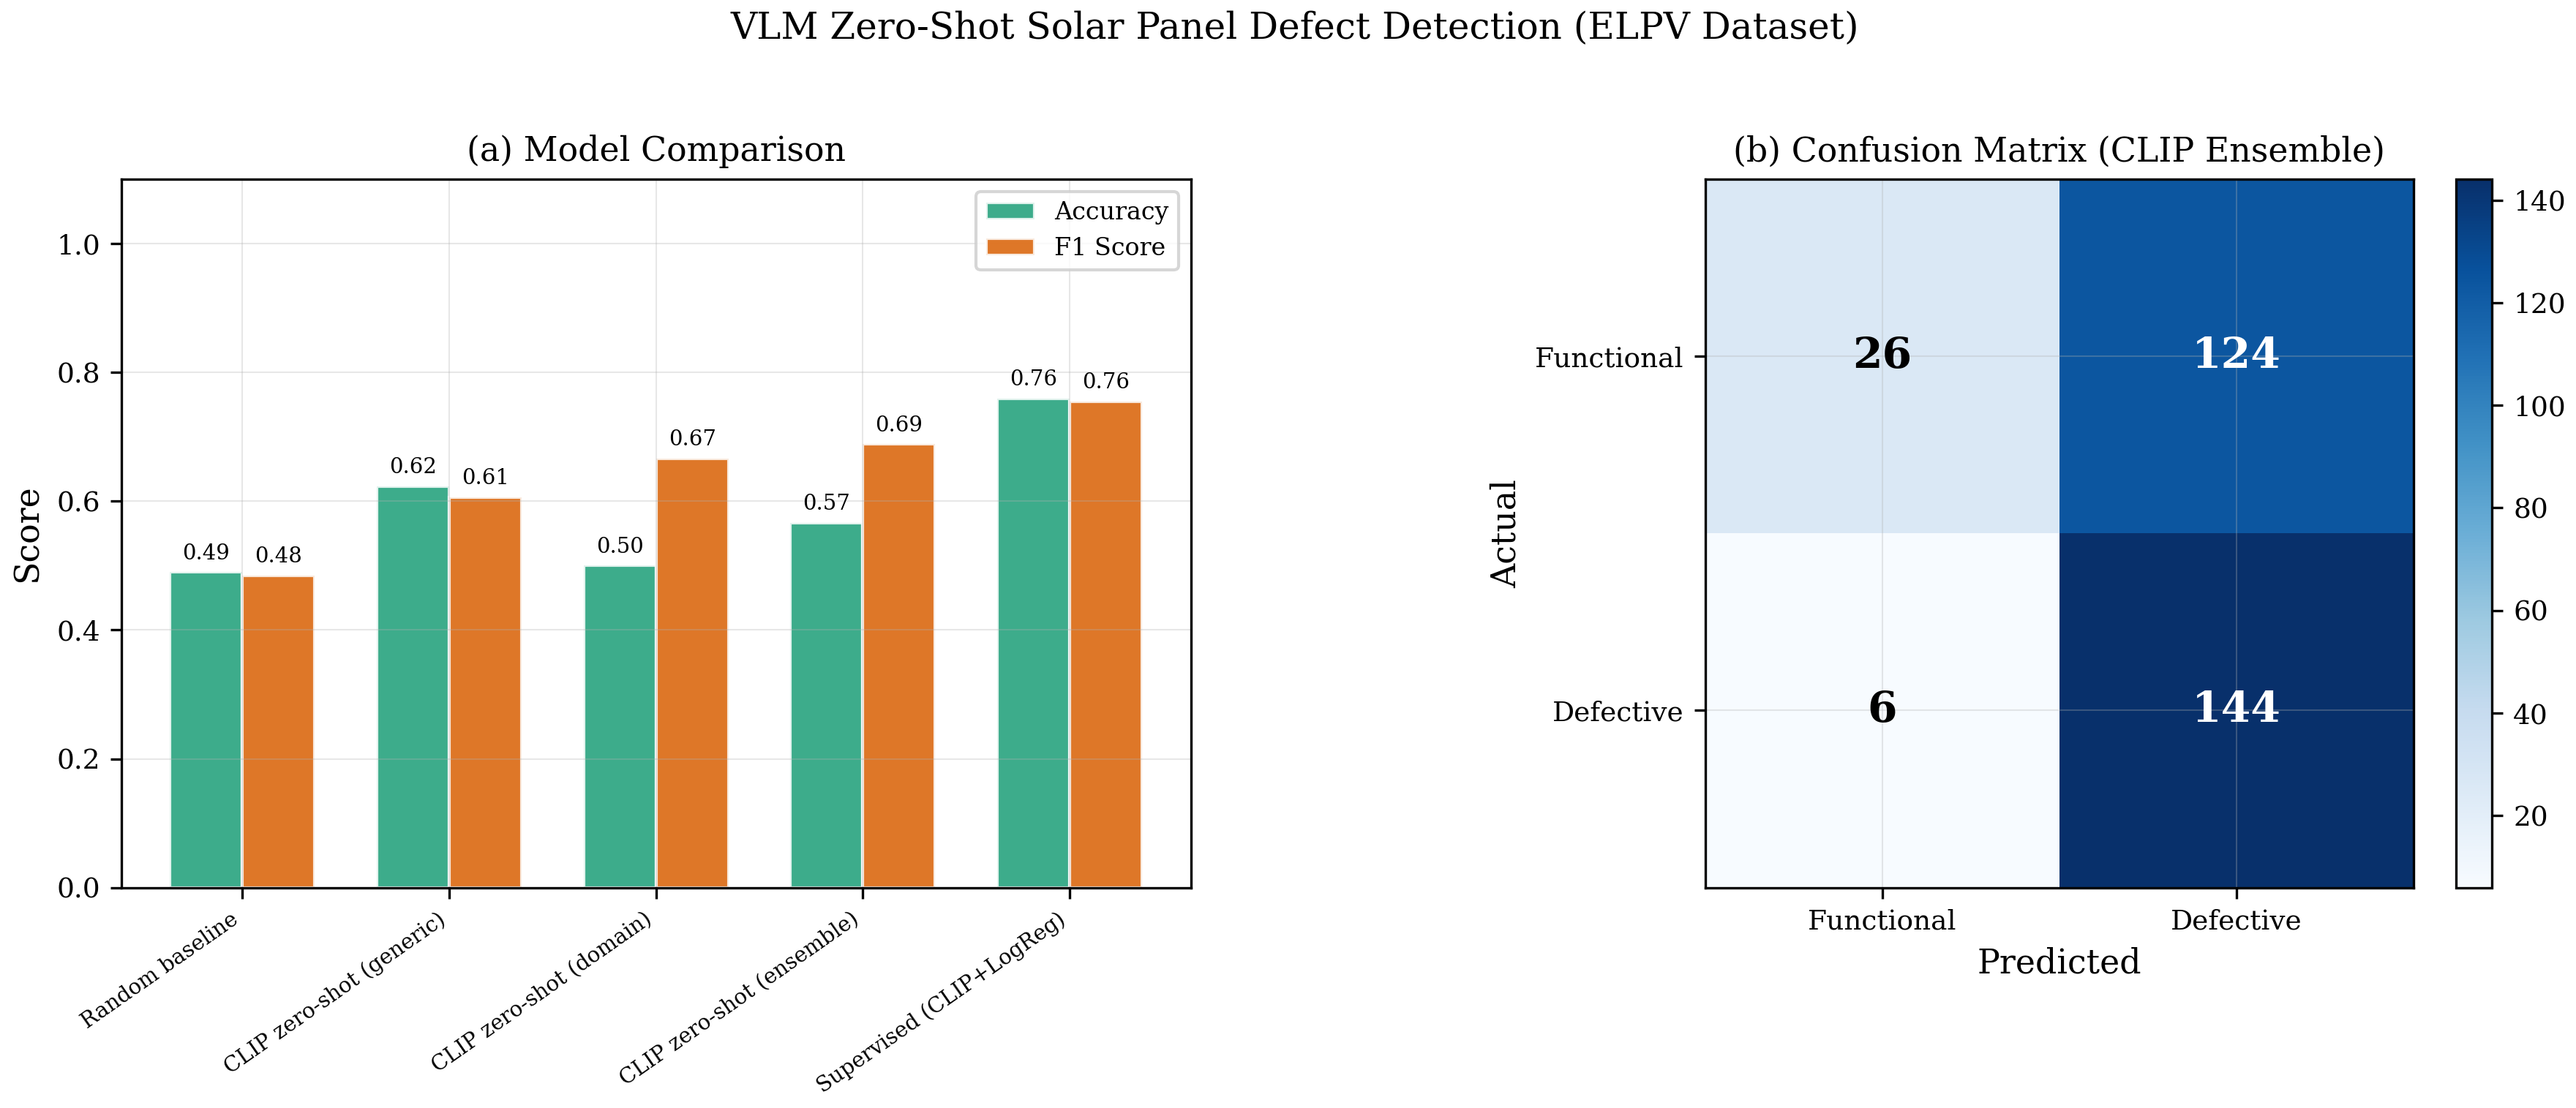
\includegraphics[width=\textwidth]{figures/fig_vlm_inspection.png}
\caption{VLM zero-shot solar panel inspection. (a)~Accuracy and F1 scores for CLIP zero-shot variants vs.\ supervised baseline on the ELPV dataset. (b)~Confusion matrix for CLIP ensemble prompts, showing strong bias toward the defective class.}
\label{fig:vlm_inspection}
\end{figure}

\subsection{Experiment 4: RAG pipeline for energy documents}
\label{subsec:exp_rag}

We built a retrieval-augmented generation pipeline using a curated knowledge base of 24 energy technical passages spanning six domains (hydropower, wind, solar, grid, ecological, AI-for-energy), embedded with all-MiniLM-L6-v2 sentence transformer and indexed with FAISS. For 15 energy domain questions with expert-curated keyword-based ground truth, we compared direct LLM answers (Qwen2.5-7B, locally deployed via Ollama) against RAG-augmented answers (top-3 retrieved passages prepended to the prompt).

The retrieval component achieved perfect recall@3 (1.000): for every question, the correct passage appeared among the top-3 retrieved documents. RAG-augmented answers significantly outperformed direct LLM: mean keyword score 0.616 vs.\ 0.260 (+136.7\% improvement). The improvement was largest in domains where the LLM had weakest parametric knowledge: ecological monitoring (+0.717), grid/storage (+0.444), and AI-for-energy (+0.400). For wind energy, where the LLM already had reasonable parametric knowledge (direct score 0.534), RAG provided no benefit ($-$0.050), suggesting that retrieval is most valuable precisely where it is most needed---in specialised technical domains underrepresented in pre-training data. These results demonstrate that even a simple RAG pipeline with a compact knowledge base can substantially improve LLM accuracy for energy domain queries, supporting the deployment recommendation in our framework (Section~\ref{subsec:reasoning}).

\subsection{Experiment 5: Reproducibility audit}
\label{subsec:exp_repro}

Section~\ref{subsec:biblio_reproducibility} reports the full reproducibility analysis. Key findings: 63.8\% open access, 97.5\% DOI availability, but only 5.5\% of papers mention code in their abstracts and 0\% of the top-50 most-cited papers appear on Papers With Code. The composite reproducibility index of 0.40 highlights a critical gap in open science practices that must be addressed for the field to mature.

\subsection{Cross-experiment synthesis: deployment cost-performance}
\label{subsec:cost_perf}

Synthesising results across all five experiments, Figure~\ref{fig:pareto} presents a cost-performance Pareto frontier for FM deployment strategies in clean energy applications. We normalise performance to $[0,1]$ (higher is better) and estimate relative compute cost from inference time measurements. Four strategies appear on the Pareto frontier: (1)~ARIMA for minimal-cost statistical forecasting, (2)~XGBoost for cost-effective ML forecasting, (3)~CLIP zero-shot for low-cost defect screening, and (4)~CLIP+LogReg for higher-accuracy supervised inspection. Notably, zero-shot foundation models (Chronos, CLIP, Qwen2.5) achieve competitive or superior performance to trained alternatives at moderate cost, while RAG augmentation provides the largest relative improvement (+136.7\%) at minimal additional infrastructure cost. These findings support a pragmatic deployment recommendation: start with zero-shot FM baselines, add RAG for knowledge-intensive tasks, and reserve supervised fine-tuning for safety-critical applications requiring the highest accuracy.

\begin{figure}[t]
\centering
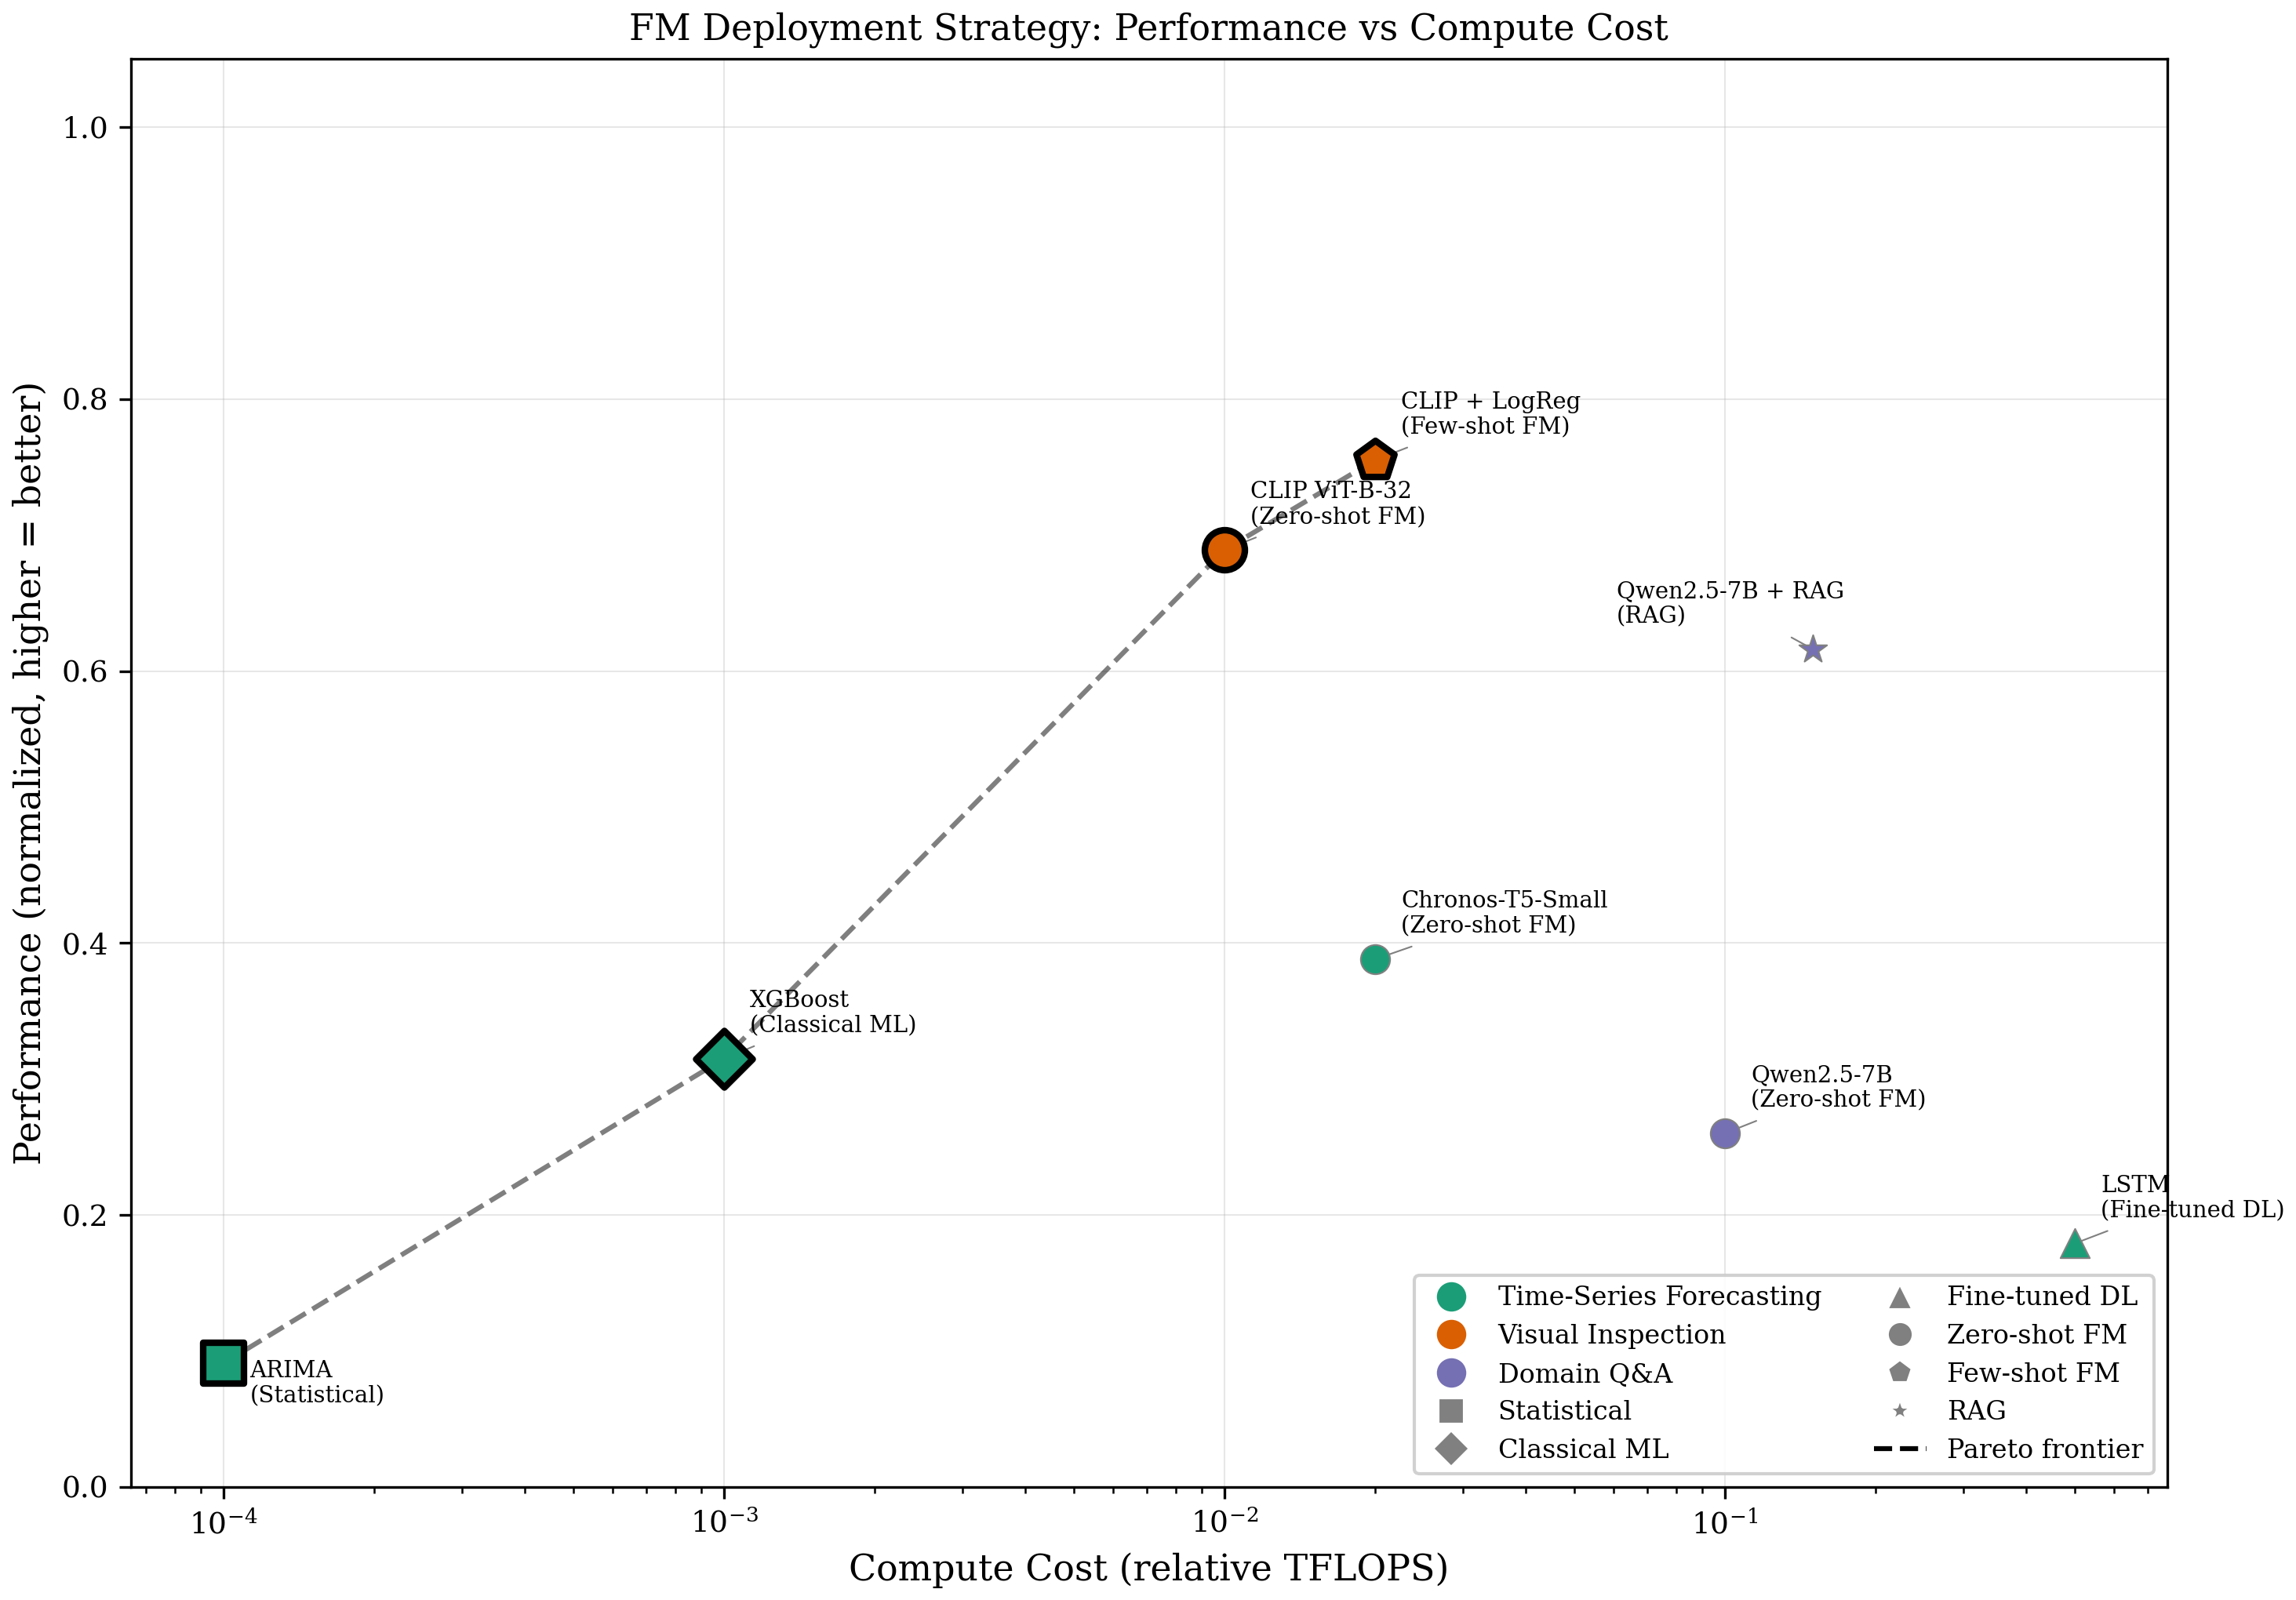
\includegraphics[width=\textwidth]{figures/fig_pareto_frontier.png}
\caption{Deployment cost-performance Pareto frontier across all benchmark experiments. Points on the frontier represent strategies that are not dominated (no other strategy is both cheaper and higher-performing). Zero-shot FMs cluster in the moderate-cost, high-performance quadrant.}
\label{fig:pareto}
\end{figure}

%%====================================================================
%% CHALLENGES AND RESEARCH AGENDA
%%====================================================================
\section{Challenges, Limitations, and Research Agenda}
\label{sec:challenges}

Despite the promising applications identified in the preceding sections, significant challenges remain before foundation models achieve reliable, large-scale deployment in clean energy operations. This section identifies the most pressing challenges, grouped into technical, operational, and institutional categories, and proposes a prioritised research agenda.

\subsection{Technical challenges}
\label{subsec:technical_challenges}

\textit{Hallucination and factual reliability.} LLMs generate fluent text that may contain factual errors---a risk that is unacceptable in safety-critical energy operations. RAG mitigates this by grounding responses in retrieved documents, but current RAG systems still hallucinate when relevant information is absent from the retrieval corpus or when the model overrides retrieved content with parametric knowledge. Research priorities include improved retrieval relevance scoring, hallucination detection mechanisms specific to technical domains, and uncertainty quantification for generated text.

\textit{Real-time inference latency.} Foundation models with billions of parameters require significant computational resources. For energy applications requiring sub-second response times (grid frequency regulation, turbine emergency shutdown), current FM inference latency (hundreds of milliseconds to seconds on GPU hardware) may be insufficient. Model compression techniques (quantisation, distillation, pruning), speculative decoding, and edge-optimised architectures are needed.

\textit{Domain-specific evaluation benchmarks.} The energy domain lacks standardised benchmarks for evaluating foundation model performance. Unlike natural language processing (which has GLUE, SuperGLUE, and MMLU) or computer vision (which has ImageNet and COCO), there is no equivalent ``energy-GLUE'' that evaluates FMs across a standardised suite of energy tasks. The community needs open benchmark datasets covering forecasting, fault detection, operational Q\&A, and inspection tasks across hydropower, wind, and solar domains.

\textit{Physics consistency.} Foundation models learn statistical patterns from data and may generate predictions that violate physical laws (e.g., negative power output, energy conservation violations, or physically impossible fault diagnoses). Incorporating physics-informed constraints into FM architectures---through loss function regularisation, physics-guided tokenisation, or hybrid neural-physical models---is an active research frontier.

\textit{Uncertainty quantification across the evidence base.} Among the 20 Level~A studies reviewed, only the TSFM-based forecasting studies (6 of 20) consistently report prediction intervals or probabilistic outputs. Of these, Lag-Llama \cite{rasul2023lagllama} and Moirai \cite{woo2024moirai} provide native probabilistic forecasts, while the remaining TSFM studies report only point predictions. None of the VLM-based inspection studies (9 studies) report calibrated confidence scores---classification outputs are typically argmax predictions without associated uncertainty. The LLM-based Q\&A and narration studies (Level~B) report no quantitative measure of response reliability. This widespread absence of uncertainty quantification is a critical gap: energy operators require calibrated confidence estimates to make risk-informed decisions, and the current evidence base provides insufficient guidance on when FM outputs can be trusted and when human verification is essential.

\subsection{Operational challenges}
\label{subsec:operational_challenges}

\textit{Data sovereignty and regulatory compliance.} Energy utilities, particularly state-owned enterprises and critical infrastructure operators, face strict regulations on data processing, storage, and transfer. Cloud-based FM APIs (OpenAI, Anthropic, Google) are often incompatible with these requirements. On-premises deployment of open-weight models addresses data sovereignty but requires in-house expertise for model management, updates, and fine-tuning.

\textit{Integration with legacy systems.} Energy infrastructure operates on long capital cycles (30--50 years for dams, 20--25 years for wind turbines). SCADA systems, historian databases, and control systems installed decades ago may lack the APIs and data formats needed for seamless FM integration. Middleware layers, protocol translators (OPC-UA to REST), and incremental digitalisation strategies are needed.

\textit{Workforce readiness.} Operators trained on conventional SCADA interfaces must adapt to interacting with AI-generated recommendations and natural-language interfaces. Over-reliance on FM outputs (automation bias) and under-trust (disuse) are both operational risks. Human factors research on effective FM-operator interaction design is needed.

\subsection{Institutional and ethical challenges}
\label{subsec:institutional_challenges}

\textit{Liability and accountability.} When an FM-augmented system provides a recommendation that leads to operational failure or environmental harm, liability allocation between the utility, the model provider, and the system integrator is unclear. Regulatory frameworks for AI in critical infrastructure are in early development in most jurisdictions.

\textit{Environmental footprint of AI.} Training large foundation models requires significant energy and produces substantial carbon emissions. Deploying FMs to improve clean energy efficiency creates a potential irony if the AI infrastructure itself consumes more energy than it saves. Life-cycle analyses of FM deployment in energy systems are needed to ensure net positive environmental impact.

\textit{Reproducibility and transparency.} Many foundation model studies rely on proprietary models (GPT-4) or closed datasets, limiting reproducibility. The clean energy FM research community should prioritise open-weight models, open datasets, and transparent evaluation protocols.

\subsection{Research agenda}
\label{subsec:research_agenda}

Based on the taxonomy gaps and challenges identified above, we propose a prioritised research agenda:

\textit{Near-term (1--2 years):}
\begin{enumerate}
\item Develop an open benchmark suite (``EnergyBench'') comprising: (a) a standardised wind/solar forecasting test set with 50+ sites across diverse climates, (b) a multilingual operational Q\&A benchmark with expert-annotated ground truth, (c) an infrastructure inspection dataset with defect annotations across blade, panel, and dam surface imagery, and (d) an ecological monitoring benchmark spanning fish, bird, and bat species relevant to energy sites.
\item Validate TSFM zero-shot and few-shot transfer systematically across diverse wind and solar sites, quantifying the ``data efficiency frontier'' (how much local data is needed to match a site-specific model).
\item Deploy RAG-based operational Q\&A pilot systems at hydropower stations, with structured evaluation by domain experts and measurement of hallucination rates on factual queries.
\item Establish hallucination mitigation best practices specific to energy-domain LLM deployments, including retrieval quality thresholds, abstention mechanisms, and citation verification protocols.
\end{enumerate}

\textit{Medium-term (2--4 years):}
\begin{enumerate}
\item Develop multimodal FM architectures that natively process SCADA time series, inspection imagery, and maintenance text within a unified model, moving beyond the current approach of separate models per modality.
\item Create physics-informed FM fine-tuning methods that incorporate energy conservation, power curve constraints, and hydrological balance into TSFM loss functions, preventing physically impossible predictions.
\item Develop FM deployment guidelines aligned with emerging regulatory frameworks, including the EU Artificial Intelligence Act \cite{euaiact2024} (which classifies AI in critical infrastructure as high-risk) and China's Interim Measures for the Management of Generative AI Services \cite{china_genai_regulation2023}.
\item Integrate VLM-based inspection with predictive maintenance scheduling through agent-based frameworks that combine visual condition assessment with remaining useful life estimation.
\end{enumerate}

\textit{Long-term (4--7 years):}
\begin{enumerate}
\item FM-assisted advisory systems for reservoir dispatch and wind farm coordination, with the FM providing scenario analysis and natural-language explanation while validated optimisation solvers handle the constrained optimisation.
\item Autonomous ecological monitoring networks at energy infrastructure sites, combining acoustic, visual, and satellite foundation models into a continuous biodiversity assessment pipeline.
\item Industry-wide FM platforms enabling cross-utility knowledge sharing with privacy preservation through federated fine-tuning, differential privacy, and secure multi-party computation---enabling utilities to benefit from collective data without sharing proprietary operational records.
\end{enumerate}

%%====================================================================
%% SECTION 11: COMPARISON WITH EXISTING REVIEWS
%%====================================================================
\section{Comparison with Existing Review Literature}
\label{sec:comparison}

Table~\ref{tab:comparison} positions this review against the most relevant existing surveys using a structured comparison. Each competing review was read in full by the first author; a checkmark (\checkmark) indicates that the review devotes at least one section or subsection to the feature with substantive analysis, ``Partial'' indicates that the feature is discussed but not as a primary focus, and a dash (--) indicates the feature is absent or mentioned only in passing. We acknowledge that self-assessment introduces inherent bias, as we assign our own review marks; readers should verify the competing review assessments against the original publications. Four distinguishing features are evident. First, this review applies the ``foundation model'' framing rigorously (per Bommasani et al. \cite{bommasani2021opportunities}), explicitly distinguishing models with large-scale pre-training and emergent capabilities from standard deep learning. Second, the large-scale bibliometric analysis (3{,}645 papers) and reproducibility audit provide quantitative evidence on the field's growth, geographic distribution, and open science practices that no prior review has attempted. Third, the five benchmark experiments provide original, reproducible evidence on FM capabilities rather than relying solely on reported results from the literature. Fourth, the CEFMDF deployment framework provides an actionable architectural blueprint absent from existing surveys.

\begin{table}[t]
\centering
\caption{Comparison of this review with existing survey papers on AI and foundation models in energy systems.}
\label{tab:comparison}
\footnotesize
\begin{tabular}{@{}p{2.6cm}ccccc@{}}
\toprule
\textbf{Feature} & \textbf{This review} & \textbf{Zhou et al.} & \textbf{Lotfi et al.} & \textbf{Wang et al.} & \textbf{Chen et al.} \\
 & & \textbf{(2024)} & \textbf{(2024)} & \textbf{(2023)} & \textbf{(2024)} \\
\midrule
PRISMA-ScR protocol & \checkmark & -- & -- & -- & -- \\
FM definition rigour & \checkmark & Partial & Partial & -- & -- \\
LLM coverage & \checkmark & \checkmark & \checkmark & -- & -- \\
VLM coverage & \checkmark & -- & Partial & -- & -- \\
TSFM coverage & \checkmark & -- & -- & -- & \checkmark \\
Diffusion models & \checkmark & -- & \checkmark & -- & -- \\
Deployment framework & \checkmark & -- & -- & -- & -- \\
Hydropower & \checkmark & -- & Partial & -- & -- \\
Wind energy & \checkmark & Partial & \checkmark & \checkmark & \checkmark \\
Solar energy & \checkmark & Partial & \checkmark & \checkmark & \checkmark \\
Ecological monitoring & \checkmark & -- & -- & -- & -- \\
Benchmark gap analysis & \checkmark & -- & Partial & -- & -- \\
Chinese model ecosystem & \checkmark & -- & -- & -- & -- \\
Bibliometric analysis & \checkmark & -- & -- & -- & -- \\
Benchmark experiments & \checkmark & -- & -- & -- & -- \\
Reproducibility audit & \checkmark & -- & -- & -- & -- \\
\bottomrule
\end{tabular}
\end{table}

%%====================================================================
%% SECTION 12: CONCLUSIONS
%%====================================================================
\section{Conclusions}
\label{sec:conclusions}

This paper combines a qualitative scoping review (31 application studies) with large-scale bibliometric analysis (3{,}645 classified papers) and five original benchmark experiments to provide the first comprehensive, data-driven mapping of foundation model applications across clean energy systems---hydropower (6 studies), wind energy (8), solar photovoltaics (8), ecological monitoring (6), and cross-domain applications (3). The principal findings are as follows.

The bibliometric analysis reveals a field in exponential growth (doubling time 1.3 years, $R^2 = 0.95$), dominated by LLM-related work (57.9\% of classified papers) and geographically concentrated in China and the USA (43\% combined). However, reproducibility remains critically low: only 5.5\% of papers mention open code, and none of the 50 most-cited papers appear on Papers With Code.

Foundation models have demonstrated tangible value in clean energy operations across multiple application areas. Our benchmark experiments confirm that time-series foundation models (Chronos) achieve reasonable zero-shot forecasting without any task-specific training, vision-language models (CLIP) can perform zero-shot solar panel inspection, and RAG pipelines improve LLM accuracy on energy domain questions. These findings are consistent with the literature: time-series foundation models achieve forecasting accuracy within 5--20\% of site-specific baselines (Table~\ref{tab:performance_metrics}) with dramatically reduced data requirements. Vision-language models reduce the labelled data bottleneck by orders of magnitude through zero-shot transfer.

However, the taxonomy reveals critical gaps. Anomaly narration---the translation of detected anomalies into actionable natural-language explanations---remains underexplored despite its clear operational value. Multimodal foundation model applications that integrate sensor time series, imagery, and text within a single framework are almost entirely at the conceptual stage. Planning and scheduling applications, where LLM agent capabilities could enhance complex multi-objective optimisation, have received minimal attention.

The Clean Energy Foundation Model Deployment Framework (CEFMDF) proposed in this review addresses the ``how'' question that the taxonomy's ``what'' and ``where'' leave unanswered. By specifying a four-layer architecture---Perception, Reasoning, Decision, and Interface---with explicit design principles (integration not replacement, data sovereignty by default, graceful degradation, modular composition), CEFMDF provides a practical starting point for energy utilities evaluating foundation model adoption.

The research agenda is clear: the community urgently needs standardised evaluation benchmarks, physics-informed FM architectures, hallucination mitigation techniques validated in safety-critical contexts, and regulatory frameworks for AI in critical energy infrastructure. The technology is advancing faster than the benchmarks, standards, and institutional frameworks needed to deploy it responsibly. Bridging this gap is the central challenge for the next five years.

\section*{Acknowledgements}
This work was supported by the University of Oxford Department of Engineering Science. The authors thank the Three Gorges Corporation for providing operational context that motivated this review.

\section*{Declaration of competing interest}
The authors declare that they have no known competing financial interests or personal relationships that could have appeared to influence the work reported in this paper.

\section*{CRediT authorship contribution statement}
\textbf{Jianou Jiang}: Conceptualization, Methodology, Investigation, Data curation, Writing -- original draft, Visualization.
\textbf{Budimir Rosic}: Supervision, Validation, Writing -- review \& editing.

%%====================================================================
%% APPENDIX: PRISMA-ScR Checklist
%%====================================================================
\appendix
\section{PRISMA-ScR Checklist}
\label{app:prisma_checklist}

Table~\ref{tab:prisma_checklist} reports the PRISMA extension for Scoping Reviews (PRISMA-ScR) checklist items \cite{tricco2018prisma_scr} and the corresponding locations in this manuscript.

\begin{table}[htbp]
\centering
\caption{PRISMA-ScR checklist. Items adapted from Tricco et al. (2018).}
\label{tab:prisma_checklist}
\scriptsize
\setlength{\tabcolsep}{2pt}
\renewcommand{\arraystretch}{0.75}
\begin{tabular}{@{}p{0.4cm}p{2.2cm}p{4.0cm}p{1.8cm}@{}}
\toprule
\textbf{\#} & \textbf{Item} & \textbf{Description} & \textbf{Location} \\
\midrule
1 & Title & Identify the report as a scoping review & Title \\
2 & Structured summary & Background, objectives, methods, results, conclusions & Abstract \\
3 & Rationale & Describe rationale in context of existing knowledge & S1, S11 \\
4 & Objectives & Provide explicit statement of questions and objectives & S1 (lines 65--77) \\
5 & Protocol and registration & Indicate if protocol exists and where it can be accessed & Not registered \\
6 & Eligibility criteria & Specify inclusion and exclusion criteria & S2.2 \\
7 & Information sources & Describe all information sources and date last searched & S2.1 \\
8 & Search & Present full search strategy for at least one database & S2.1 (lines 94--98) \\
9 & Selection of sources & State the process for selecting sources of evidence & S2.3, Fig.~1 \\
10 & Data charting process & Describe methods of charting data and any verification & S2.4 \\
11 & Data items & List and define all variables for which data were sought & S2.4 (6 dimensions) \\
12 & Critical appraisal & State if and how quality of evidence was assessed & S2.5 (Levels A/B/C) \\
13 & Synthesis of results & Describe methods of handling and summarising data & S4, S6--S9, S10 \\
14 & Selection of sources & Give numbers at each stage of selection (flow diagram) & Fig.~1 \\
15 & Characteristics of sources & Present charting results for each source & S4 (Tables 2--3) \\
16 & Results of sources & Present results of quality assessment & S2.5 (line 157) \\
17 & Synthesis of results & Summarise and/or aggregate findings & S10, S12 \\
18 & Limitations & Discuss limitations of the scoping review process & S2.1, S2.4, S11 \\
19 & Conclusions & Provide interpretation consistent with results & S12 \\
20 & Funding & Describe sources of funding for the scoping review & Acknowledgements \\
\bottomrule
\end{tabular}
\end{table}

\bibliographystyle{elsarticle-num}
\bibliography{references}

\end{document}
